% Tento soubor nahraďte vlastním souborem s obsahem práce.
%=========================================================================
% Autoři: Michal Bidlo, Bohuslav Křena, Jaroslav Dytrych, Petr Veigend a Adam Herout 2019
\chapter{Úvod}

Pokrok v technológii a informatike nám ako spoločnosti umožňuje inováciu vo všetkých 
oblastiach. Aj pomocné vedy historické ako genealógia sa konečne v dnešnej dobe 
dočkávajú posunu vopred umožnenému aj vďaka informačným technológiám. Automatizácia 
v oblasti spracovávania a porovnávania genealogických dát môže ušetriť veľké množstvo 
potrebnej ľudskej práce. Problematikou automatizácie a inteligentného prepájania záznamov 
do rodokmeňov sa zaoberá aj práca Ing. Tušimovej \cite{formalniDP}. V tejto práci sa detailne venuje 
spracovávaniu genealogických dát z matrík narodených/pokrstených a následnému 
generovaniu grafovej databázy obsahujúcej všetky spracované osoby, mestá, záznamy 
o krste a jednotlivé vzťahy medzi všetkými spracovanými uzlami. Práca Ing. Tušimovej má 
veľký prínos pre spomínanú oblasť, pretože ju je možné použiť pre zrýchlenie a zefektívnenie 
práce pri spracovávaní genealogických dát. Avšak vždy je priestor pre zlepšenie. Práve 
tomuto sa bude venovať moja práca. 
 V prvej časti bakalárskej práce sa budeme zaoberať naštudovanými materiálmi
a teoretickými znalosťami, predovšetkým prácou Ing. Tušimovej, na ktorú táto práca 
nadväzuje. Detailnejšie si rozoberieme časť návrhu a implementácie jej práce. 
 V druhej časti práce sa pozrieme na možné vylepšenia algoritmu, ktoré by viedli ku 
presnejším výsledkom porovnávaní a klasifikovaní záznamov. Povieme si, akým spôsobom 
bude realizované pridanie podpory pre ďalšie možnosti vstupných dát, konkrétne matriky 
sobášov a matriky úmrtí a taktiež si priblížime spôsob zefektívnenia celého algoritmu.

\chapter{Naštudované materiály a teória} 
\label{struktura}
V tejto kapitole si vysvetlíme základné pojmy používané v tejto práci, formy genealogických 
záznamov, detailnejšie si priblížime prácu Ing. Tušimovej a mechanizmus spracovávania 
genealogických údajov v nej použitý. Všetky informácie použité v tejto kapitole sú prevzaté 
zo zdrojov \cite{formalniDP, britannica, kotesova, lednicka}.

\section{Kľúčové pojmy a ich vysvetlenie}
V tejto podkapitole prejdeme niekoľko základných pojmov týkajúcich sa tejto práce 
a genealógie všeobecne.
\subsection*{Genealógia}
Genealógia je pomocná veda historická zaoberajúca sa štúdiom rodín, rodinnej histórie 
a tvorbe rodokmeňov. Genealógiu v nejakej forme môžeme nájsť v každom historickom 
období, nezávisle od národa. Pred zavedením písomných záznamov išlo o orálnu tradíciu 
predávania informácií, pričom sa spoliehalo iba na pamäť ľudí a prípadné primitívne formy 
mnemotechnických pomôcok. Počiatky písomných genealogických záznamov siahajú do 
starovekého Grécka a Ríma, kde sa však ešte nedá hovoriť o genealógii ako o vednej 
disciplíne, keďže išlo skôr o vedľajšie informácie pri písaných textoch. V období stredoveku 
sa genealógovia zaoberali najmä rodinnou históriou šľachtických a kráľovských rodov 
a zostavovaním rodokmeňov týchto rodov. V modernej dobe je genealógia dostupná pre 
všetkých, vďaka jednoducho dohľadateľným záznamom, ktoré sú dostupné aj širokej 
verejnosť online alebo v archívoch. Každý sa teda môže stať genealógom, či už skúma iba 
svoju vlastnú rodinnú históriu alebo sa genealógii venuje profesionálne.

\subsection*{Matrika}
Matriky sú formou verejných záznamov, do ktorých sa zapisujú informácie slúžiace ku 
evidencii obyvateľstva. Keďže cirkev v minulosti zohrávala v spoločnosti významnú úlohu 
a podieľala sa aj na výkone práva a verejnej správy, pochádzajú prvé záznamy práve od 
cirkevných inštitúcií. Časom sa však postupne presunuli pod štátnu správu. V matrikách 
nájdeme všetky skutočnosti dôležité z hľadiska osobného stavu občana. Z tohto dôvodu 
slúžia ako hlavný zdroj genealogických informácií. Najčastejšou formou vedených matrík sú
matriky narodených (alebo krstených), matriky o uzavretých manželstvách a matriky úmrtí. 
Bližšie podrobnosti o týchto matrikách si povieme v ďalších častiach tejto kapitoly. Až do 
roku 1784 boli matriky súkromnou záležitosťou jednotlivých farností a teda nemali jednotný 
formát a často boli všetky formy matrík vedené v jednej knihe. V tomto roku však za vlády 
cisára Josefa II. vyšla séria patentov venujúca sa záležitostiam štátnej správy. Jedným 
z týchto patentov bol aj patent z 1.5.1784, ktorý zaviedol jednotný formát matrík a taktiež 
rozdelil matriky podľa formy záznamov ktoré v nej boli vedené na matriky narodených, 
matriky sobášov a matriky úmrtí. 

\subsection*{Matrika narodených/krstov}
Tieto matriky obsahovali záznamy o pôrodoch a krstoch. V lepšom prípade obsahovali 
matriky obidva údaje. Všetky údaje vedené v týchto matrikách boli dátum narodenia (alebo 
krstu), číslo domu, meno narodenej osoby, pohlavie, stav – manželský alebo nemanželský, 
náboženstvo – katolícke alebo nekatolícke, meno otca, meno matky, meno kmotra 
a v neskorších záznamoch bolo bežné taktiež meno krstiaceho duchovného a pôrodnej 
baby. 

\subsection*{Matrika úmrtí} 
Matriky úmrtí obsahovali dátum pohrebu, meno kňaza zodpovedného za zaopatrenie 
a pochovanie zosnulého, číslo domu, meno, náboženstvo, pohlavie, vek a príčinu smrti 
zosnulého. 

\subsection*{Matrika sobášov}
Údaje bežne vedené v týchto matrikách boli dátum sobáša, meno ženícha, meno nevesty, 
meno kňaza, ktorý ich sobášil a mená svedkov. V novších záznamoch sú bežné aj ďalšie údaje, 
ako bydlisko ženícha i nevesty, ich vek, náboženstvo a v prípade, že nevesta nebola plnoletá 
aj povolenie otca ku sobášu.

\section{Podkladová práca}
Táto podkapitola sa bude detailnejšie venovať diplomovej práci Ing. Tušimovej. Priblížime si 
návrh, použité technológie, implementačné detaily a výstupy práce. Všetky informácie 
použité v tejto podkapitole boli naštudované a prebrané zo zdroja \cite{formalniDP}, ktorý slúžil ako hlavný 
študijný materiál pre túto prácu.

\subsection{Návrh}
Prvou časťou práce je dátová analýza. Najprv ide teda o získanie všetkých potrebných 
údajov zo záznamu. Údaje ktoré sú pre prácu relevantné sú konkrétne:
\begin{multicols}{2}
    \begin{itemize}
        \item Meno
        \item Priezvisko
        \item Titul
        \item Pohlavie
        \item Národnosť
        \item Dátum narodenia
        \item Dátum krstu
        \item Interval dátumu narodenia
        \item Miesta kde osoba žila
        \item Vierovyznanie
        \item Dátum úmrtia
        \item Interval dátumu úmrtia
        \item Miesto úmrtia
        \item Povolanie
        \item Rodinný príslušníci
    \end{itemize}
\end{multicols}

V prípade, že v zázname chýba presný dátum, dôjde ku odhadu intervalu na základe dostupných informácií. Ak je potom pri spracovávaní ďalších záznamov získaná presnejšia hodnota dôjde ku aktualizácií intervalu a v prípade získania presnej hodnoty sa interval nahradí týmto presným dátumom. Ďalej sa využíva zhlukovanie dát, keďže významovo rovnaké mená a názvy obsiahnuté v matričných záznamoch sa často v zázname od záznamu líšili. Je preto využitá normalizácia, čo je zavedenie jednotnej formy každého mena či názvu. Použitím normalizovanej formy mien a názvov sa eliminuje množstvo chýb, ktoré 
by mohli vzniknúť používaním nenormalizovaných hodnôt.
Ďalej dochádza ku porovnávaniu jednotlivých údajov. Porovnávanie sa líši na základe typu 
údaju. Všeobecne sa porovnávanie vykonávané v práci dá rozdeliť na porovnávanie slov, 
porovnávanie dátumov, porovnávanie geografických dát, porovnávanie čísel a finálne 
porovnanie celého záznamu zostavením vektoru hodnôt z jednotlivých porovnaní. 

\subsubsection{Porovnávanie slov}
Zisťovanie podobnosti slov, ktoré nie sú normalizované je v práci realizované pomocou 
Levenshteinovej vzdialenosti. Levenshteinova vzdialenosť nám udáva editačnú vzdialenosť 
dvoch reťazcov. Ide o algoritmus pre zistenie minimálneho počtu jednoznakových operácií 
potrebných pre transformáciu jedného reťazca na druhý. Týmito operáciami sú vloženie 
znaku, mazanie znaku a substitúcia znaku.

\begin {table}[ht]
\begin{center}
\begin{tabular}{ |c|c|c|c|c|c|c|c|} 
\hline
  &            &      0     & 1          & 2          & 3          & 4          & 5          \\ \hline
  &            &            & \textbf{P} & \textbf{E} & \textbf{T} & \textbf{E} & \textbf{R} \\ \hline
0 &            & \textbf{0} &      1     &      2     &     3      &      4     &      5     \\ \hline
1 & \textbf{P} &      1     & \textbf{0} &      1     &     2      &      3     &      4     \\ \hline
2 & \textbf{E} &      2     &      1     & \textbf{0} &     1      &      2     &      3     \\ \hline
3 & \textbf{T} &      3     &      2     &      1     &\textbf{0}  &      1     &      2     \\ \hline
4 & \textbf{R} &      4     &      3     &      2     &     1      & \textbf{1} &      2     \\ \hline
5 & \textbf{A} &      5     &      4     &      3     &     2      &      2     & \textbf{2} \\ \hline

\hline
\end{tabular}
\caption {Príklad určenia Levenshteinovej vzdialenosti dvoch reťazcov} \label{levenshtein}
\end{center}
\end {table}

V tabuľke \ref{levenshtein} prevzatej zo zdroja \cite{formalniDP} vidíme príklad určenia Levenshteinovej vzdialenosti reťazca \textit{Peter} a reťazca \textit{Petra}. Vzdialenosť týchto dvoch reťazcov je v tomto prípade 2, keďže pre transformáciu 
prvého reťazca na druhý je nutné použiť 2 jednoznakové operácie substitúcie. Podobnosť 
dvoch reťazcov vypočítaná pomocou Levenshteinovej vzdialenosti vyzerá následovne:

\begin{equation*}
    sim_{levenshtein}(s_1,s_2) =  1.0 - \frac{ dist_{levenshtein}(s_1,s_2)}{ max(|s_1|,|s_2|)}
\end{equation*}
\newpage
\textit{sim\textsubscript{levenshtein}} udáva výslednú podobnosť reťazcov \textit{s\textsubscript{1}} a \textit{s\textsubscript{2}}. Tú získame pomocou podielu
Levenshteinovej vzdialenosti reťazcov \textit{dist\textsubscript{levenshtein}} a maxima \textit{max} z dĺžok reťazcov a následným odčítaním hodnoty od 1. Výsledné hodnoty sa teda budú blížiť 1 pri vysokej
podobnosti reťazcov a 0 pri nízkej podobnosti.

\begin{equation*}
    sim_{levenshtein}(s_1,s_2) = 
\begin{cases} 1.0  &  ak \ s_1 = s_2 \\
              0.0  &  ak \ s_1 \neq s_2. \end{cases}
\end{equation*}  

\subsubsection{Porovnanie dátumov}
Pre porovnávanie dátumov sa okrem Levenshteinovej vzdialenosti prístup kombinuje
s porovnávaním pomocou porovnávania veku, pričom sa nakoniec použije hodnota s vyššou
podobnosťou dvoch údajov. Pre porovnávanie pomocou veku je nutné určiť hodnotu
tolerancie v percentách \textit{apc\textsubscript{max}}, kvôli častým nepresným údajom z minulosti. Následne sa
určí vekový rozdiel v percentách \textit{apc} (age percentage difference).

\begin{equation*}
    apc =  \frac{ |d_1 - d_2|}{ max(|d_1|,|d_2|)} \cdot 100
\end{equation*}

\textit{d\textsubscript{1}} a \textit{d\textsubscript{2}} predstavujú hodnoty veku. Na základe rozdielu je určená podobnosť veku.

\begin{equation*}
    sim_{age} = 
\begin{cases} 1.0 -  \frac{ apc}{ apc_{max}} &  ak \quad apc < apc_{max} \\
              0.0  &  inak. \end{cases}
\end{equation*}

Okrem porovnávania veku sa používa kontrola dátumov, keďže častou chybou v zápisoch
bolo prehodenie údajov o dni a mesiaci. Preto v prípade, že hodnota o mesiaci presahuje 12
a hodnota údaju o dni nepresahuje túto hodnotu, predpokladá sa zamenenie týchto údajov.

\subsubsection{Porovnanie geografických dát}
Ďalšou metódou porovnávania použitou v práci je porovnávanie geografických súradníc. Tu
sa meria vzdialenosť medzi miestami pozdĺž zemského povrchu v kilometroch. Čím bližšie sú
miesta dvoch porovnávaných osôb, tým je vyššia pravdepodobnosť, že sa jedná o tú istú
osobu. V prípade, že údaj o presnej adrese nie je dostupný, ale podarí sa vyhodnotiť
napríklad iba región, porovnávanie je uskutočnené od stredu regiónu. V tomto prípade ide
však iba o približnú hodnotu a údaj a pri porovnávaní je mu priradená nižšia váha.

\subsubsection{Porovnanie čísel}
Tento spôsob porovnávania je použitý iba pri porovnávaní čísla ulice a je ďalej kombinovaný
s Levenshteinovou vzdialenosťou. Podobnosť čísel sa vypočíta nasledujúcim spôsobom:

\begin{equation*}
    sim_{num} = 
\begin{cases} 1.0 -  \frac{ |n_1 - n_2|}{ d{max}} &  ak \quad |n_1 - n_2| < d_{max} \\
              0.0  &  inak. \end{cases}
\end{equation*}

Kde \textit{n\textsubscript{1}} a \textit{n\textsubscript{2}} predstavujú porovnávané čísla a \textit{dmax} predstavuje maximálny tolerovaný
rozdiel medzi nimi.

\subsubsection{Porovnanie záznamov}
Záznamy sa skladajú z viacerých atribútov rôznych typov a predstavujú informácie o jednej
osobe. Pre porovnanie týchto atribútov sú použité vyššie spomínané metódy. Pre následné
porovnanie celých záznamov je zostavený porovnávací vektor z jednotlivých hodnôt
porovnávaní atribútov. Jednotlivým atribútom sú potom priradené váhy, ktorými sa
prislúchajúca hodnota porovnania pred sčítaním násobí.

\begin {table}[ht]
\begin{center}
\resizebox{\columnwidth}{!}{%
\begin{tabular}{ |c||c|c|c|c|c|c|c|} 
\hline
ID     & Meno     & Priezvisko    & Pohlavie & Dátum narodenia &    Č. domu & Názov ulice   &  Mesto    \\
\hline
a1     & alica    & mlynárová     & žena     &  18.10.1956     &        15  & božetechova  & brno     \\    
a2     & alica  & mikuláková    & žena     &  18.10.1958     &        68  & dožetekova   & břeclav   \\   
\hline
       & 1.0      & 0.0           & 1.0      &         0.87    &       0.0  & 0.73          & 0.0  \\   
\hline
\end{tabular}
}
\caption {Príklad vzniknutého porovnávacieho vektoru dvoch osôb} \label{tab_vektor}
\end{center}
\end {table}

\subsubsection{Klasifikácia}
Aby sme určili vzťah ktorý prepája dve osoby, je nutné najprv zistiť či nejde o tú istú osobu.
To overíme porovnaním pomocou atribútov. Dvojicu porovnávaných osôb si označíme ako \textit{r\textsubscript{i}} a \textit{r\textsubscript{j}}. Po sčítaní všetkých hodnôt výsledného porovnávacieho vektoru týchto osôb dostávame
hodnotu celkovej zhody \textit{SimSum}[\textit{r\textsubscript{i}, r\textsubscript{j}}]. Na základe tejto hodnoty a nastaviteľných prahov \textit{t\textsubscript{u}} a \textit{t\textsubscript{l}} vieme kategorizovať dvojicu ako zhodu, potencionálnu zhodu a nezhodu.

\begin{equation*}
SimSum[r_i,r_j] \geq t_u \implies r \rightarrow Zhoda, \\
\end{equation*}
\begin{equation*}
\quad \quad t_l < SimSum[r_i,r_j] < t_u \implies r \rightarrow Potencionálna \quad zhoda, \\
\end{equation*}
\begin{equation*}
SimSum[r_i,r_j] \leq t_l \implies r \rightarrow Nezhoda
\end{equation*}

Táto klasifikácia, však neberie do úvahy jednotlivé váhy atribútov. Preto je nutné dopočítať
tieto váhy.

\subsubsection{Pravdepodobnostná klasifikácia}

Práca používa pravdepodobnostnú klasifikáciu predstavenú v práci Ivana Fellegiho a Alana
Suntera z roku 1969 \cite{linkage}. Sú zavedené dve populácie \textit{A} a \textit{B} ktorým prislúchajú prvky \textit{a} a \textit{b}
v tomto poradí, pričom sa predpokladá, že existujú prvky, ktoré sú pre populácie \textit{A} a \textit{B}
spoločné. Následne si zadefinujeme množinu usporiadaných dvojíc definovanú následovne:

\begin{equation*}
    a~\times B = \{(a,b): a~\in A, b \in B\}
\end{equation*}

Táto množina je výsledkom zjednotenia dvoch disjunktných množín, konkrétne množiny
reprezentujúcej zhodné dvojice, teda prvky (v našom prípade osoby) sa zhodujú

\begin{equation*}
   M = \{(a,b): a=b, a~\in A, b \in B\}
\end{equation*}

a množiny reprezentujúcej nezhodné dvojice

\begin{equation*}
    U = \{(a,b): a\neq b, a~\in A, b \in B\}
\end{equation*}
\newpage
Pri každej dvojici máme už spomínaný porovnávací vektor zložený z hodnôt porovnaní
jednotlivých atribútov. Pravdepodobnosť zhody sa potom určí ako podmienená
pravdepodobnosť zhodných a nezhodných údajov v zázname.

\begin{equation*}
    R =  \frac{P(\gamma \in \Gamma| r \in M)}{P(\gamma \in \Gamma| r \in U)}
\end{equation*}

Pomocou tejto pravdepodobnosti a prahov určíme kategóriu do ktorej porovnávané osoby
patria.

\begin{equation*}
R \geq t_u \implies r \rightarrow Zhoda, \\
\end{equation*}
\begin{equation*}
\quad \quad t_l < R < t_u \implies r \rightarrow Potencionálna \quad zhoda, \\
\end{equation*}
\begin{equation*}
R \leq t_u \implies r \rightarrow Nezhoda
\end{equation*}

Táto klasifikácia je základom pravdepodobnostného prepájania záznamov.

Pri predpoklade, že tieto pravdepodobnosti sú pre jednotlivé atribúty záznamov nezávislé, je
možné každému atribútu vypočítať váhu. Váha atribútu \textit{w\textsubscript{i}} pre atribút \textit{i} sa vypočíta na
základe pravdepodobnosti \textit{m\textsubscript{i}}, ktorá udáva pravdepodobnosť, že dva záznamy majú rovnakú
hodnotu tohto atribútu kvôli tomu že sa jedná o zhodné záznamy

\begin{equation*}
m_i = P ([a_i = b_i, a~\in A, b \in B] | r\in M) \\
\end{equation*}

a pravdepodobnosti \textit{u\textsubscript{i}}, ktorá udáva pravdepodobnosť toho, že dva záznamy majú rovnakú hodnotu atribútu aj napriek tomu, že sa jedná o záznamy, ktoré sa nezhodujú.

\begin{equation*}
u_i = P ([a_i = b_i, a~\in A, b \in B] | r \in U), \\
\end{equation*}

Váha \textit{w\textsubscript{i}} atribútu \textit{i} je potom určená nasledovne:

\begin{equation*}
    w_{i} = 
\begin{cases} log_2  \frac{ m_i}{u_i}  &  ak \quad a_i = b_i, \\
              log_2  \frac{ 1- m_i}{1 - u_i}  &  a_i \neq b_i \end{cases}
\end{equation*}

\subsection{Použité technológie}

V tejto podkapitole si stručne povieme niečo o technológiách použitých v implementácii.

\subsubsection{Python 3}
Práca je implementovaná v skriptovacom jazyku python 3, ktorý je efektívny a jednoduchý na
použitie. Jedná sa o interpretovaný, dynamicky typovaný jazyk. Obsahuje veľké množstvo
knižníc, ktoré implementujú potrebné funkcionality využívané prácou.
\newpage
\subsubsection{Použité knižnice}
\begin{itemize}
    \item Levenshtein - výpočet Levenshteinovej editačnej vzdialenosti slov
    \item geopy – výpočet vzdialenosti medzi GPS súradnicami
    \item numpy – matematická knižnica
    \item datetime – práca s dátumami
    \item json – spracovanie json súborov
    \item pandas – spracovanie csv súborov
    \item time – meranie času výpočtu
\end{itemize}

\subsubsection{Vstupné dáta}

Vstupné dáta sa líšia podľa použitia programu. Je možné program spustiť v testovacom
móde, kedy je vstup načítaný z csv súborov (z angličtiny „comma separated values“), teda
súbory s hodnotami oddelenými čiarkou. V týchto súboroch je množstvo záznamov výrazne
menšie ako v použitej MySQL databáze, a preto sú ideálne na testovanie. Ďalšou formou
vstupu sú dáta z už spomenutej MySQL databázy. Pre pripojenie do databázy sa využíva
ovládač MySQL Connector/Python \cite{mysql}. Tento ovládač umožňuje jednoducho komunikovať s
databázovým serverom typu MySQL. Na dotazovanie nad databázou je využitý dotazovací
jazyk SQL. Ďalšou formou vstupu sú dáta so súradnicami GPS. Tie sú obsiahnuté
v súboroch typu JSON (JavaScript Object Notation).

\subsubsection{Grafová databáza}

Pre uloženie spracovaných dát vo forme grafu je využitá grafová databáza Neo4j. Ide
o jednu z najviac používaných grafových databáz. Pre pripojenie ku tejto databáze je použitý
ovládač Neo4j Python \cite{neo4j}. Na dotazovanie nad grafovou databázou Neo4j sa používa
dotazovací jazyk Cypher.

\subsection{Implementácia}

V tejto kapitole si stručne prejdeme implementáciu algoritmu.

\subsubsection{Načítanie dát z relačnej databázy}

V práci sa pracuje s dátami z relačnej databázy zo školského serveru \textit{fit.vutbr.cz}. Ide
o MySQL databázu obsahujúcu tabuľky pre všetky záznamy, ktoré môžu byť obsiahnuté
v matrikách narodených ako aj o matrikách samotných. Databáza ďalej obsahuje aj osobitné
tabuľky pre normalizované formy záznamov. Na prípravu a normalizáciu je použitá práca Bc.
Davida Hříbeka s názvom Poloautomatická normalizace slov z matričních záznamů \cite{normalizace}.
Prvým krokom algoritmu je pripojenie do databáz pomocou už spomenutých ovládačov.
Následne sa načítajú všetky matričné záznamy, ktoré majú formu tabuľky \textit{birth}.

\begin{figure}[h!]
  \label{birth}
  \begin{center}
  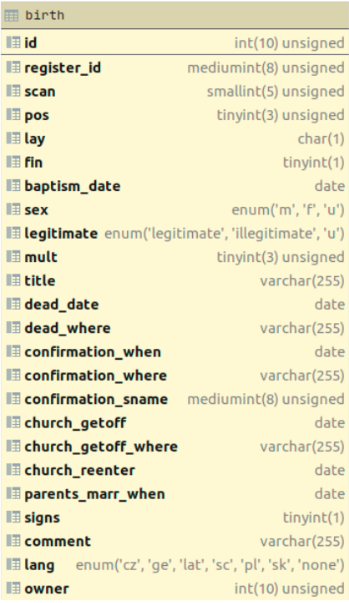
\includegraphics[width=0.5\textwidth]{obrazky-figures/birth_tabulka.png}
  \caption{Tabuľka so záznamom z matriky narodených}
  \end{center}
\end{figure}

Táto tabuľka predstavuje matričný záznam z matriky narodených. Vytvára sa nový objekt \textit{record}, do ktorého sa uložia informácie o zázname. Následne sa načítajú údaje
o prislúchajúcej matrike a uložia sa do objektu \textit{register}, ktorý reprezentuje matriku a
informácie o nej.\\
Ďalším krokom je získanie všetkých osôb. Tie sú uložené v tabuľke \textit{birthPerson}, ktorú môžete vidieť na obrázku \ref{birth}. Cez jednotlivé získané dáta o osobách sa ďalej
prechádza a získajú sa všetky potrebné informácie pre vytvorenie objektov \textit{Person}, ktoré
reprezentujú osoby figurujúce v zázname.

\subsubsection{Načítanie dát z grafovej databázy}
Z grafovej databázy sa načítavajú dáta pomocou dotazov v jazyku Cypher. Z grafovej
databázy potrebujeme získať údaje o osobách kvôli porovnaniu, preto sú dotazy cielené na
osoby a nie na záznamy. Dotazy v jazyku Cypher vrátia objekt typu slovník, ktorý má štruktúru uzla z Neo4j. V tomto objekte sú uložené všetky údaje o osobe,
s výnimkou adresy, ktorá je daná vzťahom \textit{BÝVA} medzi uzlami osôb a uzlami adries.\\
GPS súradnice sú načítané z JSON súborov a sú priradené obci ihneď potom čo sa obec
priradí osobe.

\subsubsection{Porovnávanie a klasifikácia}
Porovnanie osôb je rozdelené podľa ich pohlavia, pričom osoby s nedefinovaným pohlavím
sú porovnávané aj s mužmi aj so ženami. Prvým krokom porovnania je kontrola či osoba
v čase vzniku záznamu mohla žiť. V prípade splnenia tejto kontroly sa prechádza ku časti
základného porovnania, pri ktorom sa skontroluje meno, priezvisko, povolanie a mesto
v ktorom osoba žila. Ak sa ani jeden z týchto údajov medzi porovnávanými osobami
nezhoduje je dvojica označená ako nezhoda. V opačnom prípade sa pokračuje detailným
porovnaním ľudí. To je realizované v triede \textit{comparator}. Tu sú údaje porovnávané už
spomínanými metódami a z najlepších výsledkov jednotlivých porovnaní sa vytvára slovník \textit{comparison}. Porovnávanie často nekončí iba pri porovnaní osôb pôvodnej dvojice. Ak je to
možné porovnáva sa ďalej na základe vzťahov \textit{JE\textunderscore OTEC} a \textit{JE\textunderscore MATKA} a porovnanie
pokračuje rodičmi osoby z pôvodného porovnania. Rodič zo záznamu je vyhľadaný
v grafovej databáze a porovnanie pokračuje. Opäť vzniká objekt \textit{comparison} reprezentujúci
porovnávací vektor. Takýmto spôsobom sa pokračuje tak ďaleko ako nám povolí
spracovávaný matričný záznam. Všetky výsledky porovnaní sa ukladajú do zoznamu pre
výpočet     výsledného porovnania.\\\\
Po ukončení porovnávania sa spočítajú všetky hodnoty v slovníku \textit{comparison} vynásobené
ich príslušnými váhami, pričom hodnoty -1 označujú chýbajúci údaj a sú preto vynechané
z výpočtu. Výsledok je potom porovnaný s nastavenými prahmi a podľa toho klasifikovaný.
Návrh výsledného systému môžeme vidieť na obrázku \ref{navrh}.

\begin{figure}[h!]
  \label{navrh}
  \begin{center}
  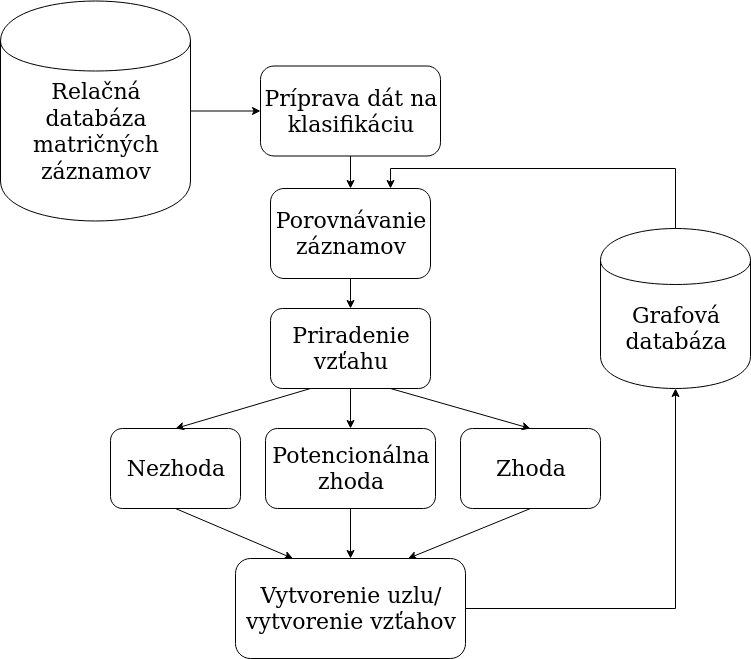
\includegraphics[width=0.7\textwidth]{obrazky-figures/navrh_riesenia2.png}
  \caption{Navrh prepojovania záznamov}
  \end{center}
\end{figure}
\newpage
\subsubsection{Uloženie záznamu}
Prvým krokom pri ukladaní záznamov je vytvorenie samotného uzlu so záznamom o krste.
Následne dôjde ku kontrole či matrika v ktorej bol záznam uložený už existuje ako uzol
v grafovej databáze. Ak nie, je vytvorený nový uzol s matrikou a ten je následne prepojený so
záznamom o krste použitím vzťahu \textit{JE\textunderscore V}. V prípade že matrika už existuje, dôjde iba ku
vytvoreniu prepojenia. Ďalej sa pokračuje podľa výsledku porovnania dvoch osôb.
V prípade že bola dvojica klasifikovaná ako nezhoda dôjde ku vytvoreniu nového uzla
s osobou. V prípade, že bola určená potencionálna zhoda dôjde taktiež ku vytvoreniu nového
uzla s osobou, ale v tomto prípade je nový uzol prepojený vzťahom \textit{POTENCIONALNI\textunderscore ZHODA} ku uzlu ku ktorému sa táto zhoda vzťahuje. V oboch prípadoch je
nutné vykonať kontrolu, či existuje uzol s adresou na ktorej daná osoba bývala. V prípade, že
adresa neexistuje je pridaná nová adresa. Údaj o adrese je zložený z uzlu obce či mesta,
ulice a popisného čísla, pričom medzi týmito uzlami funguje hierarchické prepojenie
pomocou vzťahu \textit{JE\textunderscore V}. Osoba je potom prepojená vzťahom \textit{BÝVA} na najdetailnejší údaj.
V prípade že adresa už existuje je iba vytvorené prepojenie medzi osobou a najdetailnejším
údajom z adresy. Pri vzťahu medzi adresou a osobou sa ukladá aj informácia o tom kedy
daná osoba na adrese bývala. V prípade klasifikácie dvojice osôb ako zhody dôjde ku
volaniu funkcie \textit{update\textunderscore node\textunderscore person} z triedy \textit{person.py}. Tá aktualizuje existujúci uzol o nové
hodnoty a dodatočné údaje ako napríklad povolanie, ktorých človek môže mať za život viac
uloží do listu. Po aktualizácii osoby v dôsledku zhody dôjde ku prehodnoteniu vzťahov
potencionálnych zhôd, ktoré sa môžu po doplnení nových údajov zmeniť. Ak dôjde ku
reklasifikovaniu potencionálnych zhôd na zhody proces sa opakuje. Potom čo sú vytvorené
všetky uzly začne prepájanie uzlov.\\\\
Metódou \textit{create\textunderscore connection\textunderscore with\textunderscore person\textunderscore in\textunderscore birth\textunderscore record} sa iteruje cez osoby a na základe
ich roly sú prepojené so záznamom a aj medzi sebou. Po vytvorení vzťahov medzi osobami
záznamu sa prechádza na ďalší záznam a proces sa opakuje kým nie je spracovaná celá
databáza. V tabuľke \ref{triedy} prevzanej zo zdroja \cite{formalniDP} môžeme vidieť prehľad všetkých modulov tvoriacich obsah práce.
\newpage

\begin {table}[ht]
\label{triedy}
\begin{center}
\begin{tabular}{ |c|c|} 

\hline
Triedy                           & Význam triedy \\ \hline

 main.py                         & Základný súbor, spracováva pripojenia  \\
                                 & na~databázu a~riadi testovanie \\\hline
 create\_database.py             & Hlavný algoritmus celého programu     \\   
                                 & riadi načítavanie záznamov, vytváranie grafovej\\
                                 & databázy a~spracováva výsledky porovnávania \\ \hline
 relational\_database\_birth.py  & Načítava dáta z~relačnej databázy \\ \hline
 graph\_database.py              & Načítava, aktualizuje, vyhľadáva, vytvára uzly  \\
                                 & a~prepojenia v~grafovej databáze  \\ \hline
 csv\_source.py                  & Načítava dáta z~CSV súborov  \\ \hline
 comparator.py                   & Porovnáva osoby a~vyhodnocuje výsledky,\\
                                 & obsahuje všetky metódy potrebné k~porovnávaniu  \\ \hline
 record.py                       & Trieda spravujúca záznam, obsahuje vytváranie  \\ 
                                 & uzlu, aktualizovanie uzlu, výpis informácii \\ \hline
 person.py                       & Trieda spravujúca osobu, vytváranie uzlu, \\
                                 & aktualizovanie uzlu, výpis informácií  \\ \hline
 register.py                     & Trieda spravujúca matriky, vytváranie uzlu,  \\
                                 & aktualizovanie uzlu, výpis informácií  \\ \hline
 domicile.py                     & Trieda spravujúca adresy, prehľadávanie json  \\
                                 & súborov, výpis informácií\\ \hline
 date.py                         & Trieda spravujúca dátumy \\ \hline
 get\_persons.py                 & Skript na~základe mena a~priezviská nájde všetky   \\                             
                                 & zodpovedajúce osoby uložené v~grafovej databáze\\  \hline
 get\_all\_records.py            & Skript na~základe id osoby nájde všetky záznamy \\
                                 & v~grafovej databáze, v~ktorých sa osoba nachádza \\ \hline
 get\_family\_tree.py            & Skript na~základe id osoby vypíše všetkých predkov  \\ 
                                 & a~potomkov ktorý sa nachádzajú v~grafovej databáze\\ 
\hline
\end{tabular}
\caption {Prehľad tried a~ich význam} \label{triedy}
\end{center}
\end {table}

\subsection{Dodatočné skripty}

Okrem programu realizujúceho hlavný algoritmus načítania, porovnávania, klasifikovania
a ukladania záznamov do grafovej databázy obsahuje práca Ing. Tušimovej aj ďalšie skripty
realizujúce operácie, ktoré sú z hľadiska genealogického výskumu zaujímavé. Skripty
realizujú dotazovanie nad grafovou databázou a vrátia výsledky vyhľadávania podľa
zadaných vstupných parametrov.

\subsubsection{get\textunderscore person.py}
Skript vráti výsledok vyhľadávania podľa mena a priezviska hľadanej osoby. Zobrazí všetky
informácie dostupné o tomto človeku. Prehľadávanie prebieha jednak s pôvodným menom
a aj s normalizovanou formou. Výstupom skriptu sú potom všetky informácie dostupné o danom človeku, vrátane jeho ID v grafovej databáze. To môže byť následne použité pri spúšťaní zvyšných skriptov, ktoré ako vstupný parameter vyžadujú ID osoby.

\subsubsection{get\textunderscore all\textunderscore records.py}

Skript realizuje vyhľadávanie na základe ID osoby. Skript získa a vypíše všetky záznamy
v ktorých hľadaná osoba figuruje ako aj všetky informácie o danej osobe a jej rolách
v konkrétnych záznamoch.

\subsubsection{get\textunderscore family\textunderscore tree.py}
Skript realizuje vyhľadávanie na základe ID osoby. Skript hľadá všetky osoby v prepojení \textit{JE\textunderscore MATKA, JE\textunderscore OTEC} oboma smermi. Teda hľadá predkov aj potomkov
zadanej osoby. Skript oboma smermi funguje rekurzívne a jeho výstupom je forma
rodokmeňu.

\chapter{Návrh}
V tejto kapitole si prejdeme návrh rozšírení a modifikácií, ktoré neskôr budú realizované
v rámci implementácie. Prejdeme si možnosti vylepšení algoritmu a rozšírení možností
vstupných dát. Ďalej si priblížime chyby a nedostatky zdrojovej práce, ktoré bolo nutné vyriešiť. Na záver sa pozrieme aj na možnosti optimalizácie a zvýšenia časovej efektivity skriptu.

\section{Rozšírenia}
V tejto podkapitole si ukážeme akou formou bude pôvodná práca rozšírená. Rozšírenia budú zamerná hlavne na pridanie nových typov záznamov a testovaní nových alternatív ku metrike použitej pre porovnávanie reťazcov v práci.

\subsection{Porovnávanie slov}
V tejto podkapitole sa pozrieme na rôzne alternatívy metrík použitých pri porovnávaní slov, ktoré by
mohli viesť ku lepším výsledkom, prípadne aj ku lepšej časovej efektivite programu.
Informácie v tejto podkapitole sú prevzaté zo zdroja \cite{strings}.
\newpage
\subsubsection{Jarova podobnosť}
Ak pri porovnávaní narazíme na meno, ktoré v databáze nemá normalizovanú formu,
používa sa pre určenie podobnosti mien už spomínaná Levenshteinova editačná
vzdialenosť. Existuje však prístup, ktorý by mohol byť pre porovnávanie kratších reťazcov vhodnejší a tým je Jarova podobnosť. Táto metóda je primárne určená pre kratšie reťazce a špecificky
napríklad pre mená a priezviská. Jej časová náročnosť by taktiež mala byť lepšia ako použitá
Levenshteinova editačná vzdialenosť. Metóda je podobne ako Levenshteinova vzdialenosť
založená na editačnej vzdialenosti dvoch reťazcov. Avšak okrem jednoznakových operácií
ponúkaných Levenshteinovou vzdialenosťou – vloženie, mazanie a substitúcia, pridáva
Jarova metóda ďalšiu operáciu, ktorou je transpozícia susedných znakov. Tento fakt je
obzvlášť relevantný, kvôli charakteru dát s ktorými sa táto práca zaoberá. Chyba zamenenia
susedných znakov v písaných textoch je jednou z najčastejších chýb, ktorých sa ľudia
dopúšťajú. Jarovu podobnosť \textit{sim\textsubscript{j}} dvoch reťazcov \textit{s\textsubscript{1}} a \textit{s\textsubscript{2}} vieme určiť týmto spôsobom:

\begin{equation*}
    sim\textsubscript{j} = 
\begin{cases} 0  &  ak \quad m = 0, \\
              \frac{1}{3} \cdot (\frac{m}{\mid s_{1}\mid} + \frac{m}{s_{2}} + \frac{m - t}{m})  &  inak \end{cases}
\end{equation*}

Kde $|s_{i}|$ udáva dĺžku reťazca $s_{i}$, $m$ udáva počet zhodujúcich sa znakov medzi dvoma
reťazcami a \textit{t} udáva počet transpozícií. Dva znaky patriace reťazcom \textit{s\textsubscript{1}} a \textit{s\textsubscript{2}} v tomto poradí
môžeme prehlásiť za zhodné ak sú znaky rovnaké a zároveň pre ich vzájomnú vzdialenosť \textit{d} platí nasledujúci vzťah:

\begin{equation*}
    d \leq \Bigg \lfloor \frac{max(|s_{1}|, |s_{2}|)}{2} \Bigg \rfloor - 1
\end{equation*}

Počet transpozícií je určený ako počet zhodujúcich sa znakov, ktorých sekvenčné poradie je
v porovnávaných reťazcoch odlišné vydelený dvomi.

\subsubsection{Jaro-Winklerova podobnosť}

Jaro-Winklerova podobnosť z princípu vychádza z Jarovej podobnosti, ale kladnejšie hodnotí
reťazce, ktoré sa zhodujú v prefixe až do dĺžky štyroch znakov. Pre určenie Jaro-Winklerovej
podobnosti \textit{sim\textsubscript{w}} dvoch reťazcov použijeme nasledujúci vzťah:

\begin{equation*}
    sim_{w} = sim_{j} + L \cdot p \cdot (1 - sim_{j})
\end{equation*}

Kde \textit{sim\textsubscript{j}} je hodnota Jarovej podobnosti dvoch reťazcov, \textit{L} udáva dĺžku spoločného prefixu
reťazcov až do maximálnej dĺžky prefixu 4 a \textit{p} je konštantná hodnota váhového faktoru so
štandardnou hodnotou \textit{p} = 0.1. Výraz (1 - \textit{sim\textsubscript{j}} nám udáva hodnotu Jarovej vzdialenosti (V
podstate ide o obrátenú hodnotu Jarovej podobnosti).
Táto metóda je obzvlášť relevantná, pretože ponúka výhody Jarovej podobnosti a k tomu
pozitívnejšie hodnotí reťazce so zhodným prefixom, čo je práve časté pri variáciách mien,
ktoré nemajú uloženú normalizovanú formu.

\subsubsection{Návrh implementovania metód}

Spomínané metódy je možné do programu implementovať viacerými spôsobmi. Keď
zohľadníme fakt, že metódy Jarovej vzdialenosti sú určené primárne pre kratšie reťazce a sú
obzvlášť efektívne pre porovnávanie mien, môžeme logicky dôjsť ku záveru, že bude vhodné
testovať dĺžku porovnávaných reťazcov pre určenie metódy, ktorá sa má použiť pre ich
porovnanie. Taktiež bude zohľadnený aj fakt, či ide o meno alebo priezvisko, ktoré pri
nenormalizovanej forme môžu zdieľať rovnaký prefix. Najlepší prístup bude určený
testovaním nad testovacími dátami a sledovaním presnosti klasifikácie záznamov a časovej
náročnosti výsledného algoritmu.

\begin {table}[ht]
\begin{center}
\begin{tabular}{ |c|c|} 
\hline
Premenná               & Typy porovnávania \\
\hline
 Meno                  & Presná zhoda, Levenshteinova vzdialenosť      \\
 Priezvisko            & Presná zhoda, Levenshteinova vzdialenosť      \\
 Povolanie             & Presná zhoda, Levenshteinova vzdialenosť      \\
 Mesto                  & Presná zhoda, vzdialenosť miest    \\
 Ulica                 & Levenshteinova vzdialenosť\\
 Popisné číslo         & Levenshteinova vzdialenosť, porovnávanie čísel  \\
 Dátum narodenia       & Levenshteinova vzdialenosť, kontrola dátumov,\\
                                     &  porovnanie veku\\
 Dátum (zvyšné typy)   & Levenshteinova vzdialenosť, kontrola dátumov \\
 Titul                 & Levenshteinova vzdialenosť \\
 Viera                 & Levenshteinova vzdialenosť \\
 Značky                & Presná zhoda   \\
\hline
\end{tabular}
\caption {Prehľad atribútov a spôsobov ich porovnávania} \label{porovavanie}
\end{center}
\end {table}

V tabuľke \ref{porovavanie} môžeme vidieť všetky atribúty a spôsob akým sú momentálne porovnávané. Po
zmenách v porovnávaní sa tabuľka zmení nasledujúcim spôsobom:

\begin {table}[ht]
\begin{center}
\begin{tabular}{ |c|c|} 
\hline
Premenná               & Typy porovnávania \\
\hline
 Meno                  & Presná zhoda, Jarova vzdialenosť      \\
 Priezvisko            & Presná zhoda, Jarova vzdialenosť      \\
 Povolanie             & Presná zhoda, Jarova vzdialenosť      \\
 Mesto                  & Presná zhoda, vzdialenosť miest    \\
 Ulica                 & Jarova vzdialenosť\\
 Popisné číslo         & Jarova vzdialenosť, porovnávanie čísel  \\
 Dátum narodenia       & Jarova vzdialenosť, kontrola dátumov,\\
                                     &  porovnanie veku\\
 Dátum (zvyšné typy)   & Jarova vzdialenosť, kontrola dátumov \\
 Titul                 & Jarova vzdialenosť \\
 Viera                 & Jarova vzdialenosť \\
 Značky                & Presná zhoda   \\
\hline
\end{tabular}
\caption {Prehľad atribútov a nových spôsobov ich porovnávania} \label{porovavanie_nove}
\end{center}
\end {table}

Je nutné si však uvedomiť, že pri porovnávaní niektorých atribútov bude stále možno použitá
Levenshteinova vzdialenosť, keďže tá môže byť efektívnejšia napríklad pri dlhších
reťazcoch. Bude preto nutné určiť istú formu hranice, pri ktorej sú výsledky dosiahnuté
použitím Jarovej vzdialenosti efektívnejšie, ako tie dosiahnuté použitím Levenshteinovej
vzdialenosti. Taktiež bude otestovaná efektivita Jaro-Winklerovej podobnosti a bude určený
najlepší prístup. Táto hranica bude teda určená testovaním. V tabuľke \ref{porovavanie_nove} môžeme vidieť
nové prístupy ku porovnávaniu jednotlivých atribútov.

\subsection{Ďalšie vstupné dáta}

V tejto podkapitole, si priblížime nové formy vstupných dát a urobíme základný návrh
pridania podpory.

\subsubsection{Matriky úmrtí a sobášov}

Práca Ing. Tušimovej momentálne pracuje iba s databázou obsahujúcou záznamy z matrík
narodených. Jednou z hlavných úloh mojej práce bude teda pridanie podpory pre záznamy
matrík sobášov a úmrtí. Toto bude realizované rovnakým spôsobom ako práca so
záznamami z matrík pôrodov. Pri hlavnom dotaze z funkcie v module \textit{create\textunderscore database.py}, ktorým
získavame všetky záznamy z matrík pôrodov si naberieme aj záznamy z matrík úmrtí
a sobášov. To znamená, že budeme musieť vytvoriť nové funkcie realizujúce dotazy na SQL databázu v module \textit{relational\textunderscore database\textunderscore birth.py} aby sme získali všetky ďalšie záznamy a v nich figurujúce osoby, pričom jednotlivým záznamom priradíme už predpripravený typ, podľa toho o aký
záznam pôjde. V práci bude použitá nová databáza typu MySQL s názvom demos. V tejto databáze už budú obsiahnuté aj záznamy o úmrtiach a sobášoch. Dotazy budú teda konkrétne na tabuľku \textit{burial}, v ktorej sú uložené záznamy z matrík úmrtí a tabuľku \textit{marriage}, v ktorej sú zasa záznamy o sobášoch.

\begin{longtable}{|l|c|c|c|}
 \caption{Štruktúra tabuľky burial} \label{tab:burial-structure} \\
 \hline \multicolumn{1}{|c|}{\textbf{Column}} & \multicolumn{1}{|c|}{\textbf{Type}} & \multicolumn{1}{|c|}{\textbf{Null}}\\ \hline \hline
\endfirsthead
 \caption{Štruktúra tabuľky burial (pokračovanie)} \\
 \hline \multicolumn{1}{|c|}{\textbf{Column}} & \multicolumn{1}{|c|}{\textbf{Type}} & \multicolumn{1}{|c|}{\textbf{Null}} \\ \hline \hline \endhead \endfoot
\textbf{\textit{id}} & int & No \\ \hline
register\_id & mediumint & No \\ \hline
scan & smallint & No \\ \hline
pos & tinyint & No \\ hline
lay & char(3) & Yes \\ \hline
fin & tinyint(1) & Yes \\ \hline
check\_req & tinyint(1) & Yes \\ \hline
lang & enum('CZ', 'GE', 'LAT', 'SC', 'PL', 'SK', 'NONE') & Yes \\ \hline
sex & enum('M', 'F', 'U', '[M]', '[F]') & Yes \\ \hline
dead\_born & tinyint(1) & Yes \\ \hline
viaticum\_date & char(10) & Yes \\ \hline
dead\_date & char(10) & Yes \\ \hline
burial\_date & char(10) & Yes \\ \hline
dead\_time & text & Yes \\ \hline
viaticum & tinyint(1) & Yes \\ \hline
burial\_place & text & Yes \\ \hline
death\_place & text & Yes \\ \hline
years & decimal(5,2) & Yes \\ \hline
months & decimal(5,2) & Yes \\ \hline
weeks & decimal(5,2) & Yes \\ \hline
days & decimal(5,2) & Yes \\ \hline
hours & decimal(5,2) & Yes \\ \hline
minutes & decimal(5,2) & Yes \\ \hline
death\_cause & mediumint & Yes \\ \hline
examination & tinyint(1) & Yes \\ \hline
marriage\_date & char(10) & Yes \\ \hline
marriage\_place & text & Yes \\ \hline
death\_address & int & Yes \\ \hline
birth\_address & int & Yes \\ \hline
baptised & tinyint(1) & Yes \\ \hline
legitimate & enum('legitimate', 'illegitimate', 'U') & Yes \\ \hline
marriage\_years & decimal(5,2) & Yes \\ \hline
comment & text & Yes \\ \hline
owner & int & Yes \\ \hline
score & double & Yes \\ \hline
last\_edited\_level & int & Yes \\ \hline
last\_edited\_highest\_level & int & Yes \\ \hline
 \end{longtable}

Z tabuľky \ref{tab:burial-structure} vidíme, že tabuľka záznamu o úmrtí obsahuje všetky potrebné informácie o zázname, ako jazyk v ktorom bol záznam napísaný, číslo skenu a pozícia na skene. Okrem toho záznam obsahuje aj id matriky, ktoré nám určuje matriku, z ktorej záznam pochádza. Ďalej sú tu aj relevantné informácie o zosnulom ako príčina smrti, dátum posledného zaopatrenia, úmrtia a pohrebu, pohlavie zosnulého, a fakt či nešlo o mŕtvorodené dieťa. Ďalej tabuľka samozrejme obsahuje unikátne ID, pomocou ktorého sa identifikujú všetky osoby figurujúce v danom zázname. Počet osôb figurujúcich v zázname o úmrtí je zo všetkých typov záznamov zvyčajne najnižší.

\begin{longtable}{|l|c|c|c|}
 \caption{Štruktúra tabuľky marriage} \label{tab:marriage-structure} \\
 \hline \multicolumn{1}{|c|}{\textbf{Column}} & \multicolumn{1}{|c|}{\textbf{Type}} & \multicolumn{1}{|c|}{\textbf{Null}} \\ \hline \hline
\endfirsthead
 \caption{Štruktúra tabuľky marriage (pokračovanie)} \\
 \hline \multicolumn{1}{|c|}{\textbf{Column}} & \multicolumn{1}{|c|}{\textbf{Type}} & \multicolumn{1}{|c|}{\textbf{Null}} \\ \hline \hline \endhead \endfoot
\textbf{\textit{id}} & int & No \\ \hline
register\_id & mediumint & No \\ \hline
scan & smallint & No \\ \hline
pos & tinyint & No \\ \hline
lay & char(3) & Yes \\ \hline
fin & tinyint(1) & Yes \\ \hline
check\_req & tinyint(1) & Yes \\ \hline
lang & enum('CZ', 'GE', 'LAT', 'SC', 'PL', 'SK', 'NONE') & Yes \\ \hline
banns1 & char(10) & Yes \\ \hline
banns2 & char(10) & Yes \\ \hline
banns3 & char(10) & Yes \\ \hline
marriage\_date & char(10) & Yes \\ \hline
kinship\_degree & varchar(50) & Yes \\ \hline
groom\_age\_year & decimal(5,2) & Yes \\ \hline
groom\_age\_month & decimal(5,2) & Yes \\ \hline
groom\_age\_day & decimal(5,2) & Yes \\ \hline
bride\_age\_year & decimal(5,2) & Yes \\ \hline
bride\_age\_month & decimal(5,2) & Yes \\ \hline
bride\_age\_day & decimal(5,2) & Yes \\ \hline
groom\_full\_age & char(10) & Yes \\ \hline
bride\_full\_age & char(10) & Yes \\ \hline
divorce\_date & char(10) & Yes \\ \hline
domicile & mediumint & Yes \\ \hline
unres\_descr\_num\_1 & char(10) & Yes \\ \hline
unres\_descr\_num\_2 & char(10) & Yes \\ \hline
groom\_birth\_address & int & Yes \\ \hline
groom\_dead\_address & int & Yes \\ \hline
bride\_birth\_address & int & Yes \\ \hline
bride\_dead\_address & int & Yes \\ \hline
signs & tinyint(1) & Yes \\ \hline
comment & text & Yes \\ \hline
owner & int & Yes \\ \hline
score & double & Yes \\ \hline
last\_edited\_level & int & Yes \\ \hline
last\_edited\_highest\_level & int & Yes \\ \hline
 \end{longtable}

Štruktúru tabuľky reprezentujúcej záznam o sobáši môžeme vidieť v tabuľke \ref{tab:marriage-structure}. Okrem rovnakých všeobecných informácií o samotnom zázname a matrike, ako aj v ostatných typoch záznamov, obsahuje informácie ako vek ženícha, vek nevesty, dátum sobášu, dátum rozvodu, a ďalej samozrejme aj unikátne id, pomocou ktorého dokážeme zistiť všetky osoby z tabuľky \textit{person} figurujúce v danom zázname. Naopak oproti záznamom úmrtia, obsahujú záznamy o sobášoch zvyčajne najviac figurujúcich osôb zo všetkých typov záznamov. Štruktúra tabuľky \textit{person} obsahujúcej informácie o jednotlivých osobách zo záznamu môžeme vidieť v tabuľke \ref{tab:person-structure}.

\begin{longtable}{|l|c|c|c|}
 \caption{Štruktúra tabuľky person} \label{tab:person-structure} \\
 \hline \multicolumn{1}{|c|}{\textbf{Column}} & \multicolumn{1}{|c|}{\textbf{Type}} & \multicolumn{1}{|c|}{\textbf{Null}} \\ \hline \hline
\endfirsthead
 \caption{Štruktúra tabuľky person (pokračovanie)} \\
 \hline \multicolumn{1}{|c|}{\textbf{Column}} & \multicolumn{1}{|c|}{\textbf{Type}} & \multicolumn{1}{|c|}{\textbf{Null}} \\ \hline \hline \endhead \endfoot
\textbf{\textit{id}} & int & No \\ \hline
birth\_id & int & Yes \\ \hline
marriage\_id & int & Yes \\ \hline
burial\_id & int & Yes \\ \hline
rel & enum & Yes \\ \hline
title & varchar(255) & Yes \\ \hline
sname & mediumint & Yes \\ \hline
domicile & mediumint & Yes \\ \hline
street & varchar(255) & Yes \\ \hline
descr\_num & char(10) & Yes \\ \hline
religion & enum('catholic', 'protestant', 'jew', 'none') & Yes \\ \hline
birth\_date & char(10) & Yes \\ \hline
dead & tinyint(1) & Yes \\ \hline
waif & tinyint(1) & Yes \\ \hline
category & char(1) & Yes \\ \hline
person\_relation & mediumint & Yes \\ \hline
widow & tinyint(1) & Yes \\ \hline
legitimate & enum('legitimate', 'illegitimate', 'U') & Yes \\ \hline
dead\_date & char(10) & Yes \\ \hline
work\_place & text & Yes \\ \hline
age & decimal(3,2) & Yes \\ \hline
 \end{longtable}

Každá osoba uložená v tejto tabuľke predstavuje jednu osobu figurujúcu v práve jednom zázname. Vzťah medzi osobu a záznamom je daný pomocou príslušného ID záznamu. Pôjde teda o jednu z hodnôt \textit{birth\textunderscore id}, \textit{marriage\textunderscore id} a \textit{burial\textunderscore id}. Ako hodnota v týchto stĺpcoch je použité ID záznamu, do ktorého daná osoba prináleží. Je tu preto pridaný cudzí kľúč vo forme daného ID, odkazujúceho na konkrétny záznam. Každá osoba uložená v databáze môže prináležať práve do jedného záznamu. Ďalej tabuľka obsahuje stĺpec \textit{rel}, ktorého hodnotou je jeden zo vzťahov. Tie sú reprezentované typom enum, kde sú všetky jednotlivé vzťahy vymenované. Potom tu máme informácie o dátume narodenia, smrti, veku a ďalších dodatočných informácií.
Ďalej uplatníme rovnaký postup porovnávania osôb zo záznamov ako doteraz, ale pri vytvorení nových prepojení medzi dvoma osobami a osobou a záznamom budeme musieť vytvoriť nové funkcie ktoré budú realizovať prepojenie osôb podľa ich úlohy v danom zázname. Pri práci s testovacou sadou pôjde o rovnaký postup.

\subsubsection{Rozšírenie funkcií}

V module \textit{relational\textunderscore database\textunderscore birth.py}, ktorý načítava záznamy z matrík, ale aj v ďalších častiach
programu bude potom nutné pridať kontroly zisťujúce o aký typ záznamu sa jedná. Ku každej funkcii určenej pre spracovanie záznamov o krste bude nutné vytvoriť ekvivalentnú funkciu určenú pre iný typ záznamu a prípadne na miestach, kde to bude možné, rozšíriť už existujúce funkcie tak, aby fungovali pre všetky typy záznamov. Vo výstupnej grafovej
databáze bude nutné zaviesť niekoľko nových typov uzlov. Pôjde u uzly \textit{Záznam\textunderscore o\textunderscore úmrtí} a \textit{Záznam\textunderscore o\textunderscore sobáši}. Taktiež dôjde ku pomerne veľkému rozšíreniu typu vzťahov, kde bude
nutné pridať vzťahy pre všetky nové spojenia podľa formátu nových dát. Všetky pridané vzťahy a všetky rozšírenia budú popísané ďalej v práci v časti implementácie.
\nocite{*}

\section{Analýza efektivity a problémov algoritmu}

Hlavným problémom algoritmu v pôvodnej podobe bola jeho vysoká časová náročnosť. Tá je spôsobená neustále sa zvyšujúcim počtom osôb ktoré musíme spracovať. Kvôli charakteru práce je nutné vykonávať stále viac a viac porovnaní, keďže sú osoby porovnávané spôsobom každá s každou. Pri každej porovnávanej osobe nám teda počet porovnaní vzrastie o 1. Preto môžeme hovoriť o polynomiálnej časovej komplexite a vyjadriť ju ako:

\begin{equation*}
    O(\frac{n^2 - n}{2})
\end{equation*}

kde \textit{n} je počet osôb, ktoré tvoria vstup algoritmu. Tento predpoklad môžeme učiniť, pretože počet porovnaní priamo úmerne odpovedá dobe trvania a aj keď niektoré porovnania vedú ku identifikácii zhodných osôb a ich následnému zjednoteniu, čo má síce efekt na dobu trvania programu, ide stále o zriedkavú udalosť v porovnaní s bežným scenárom pridania novej osoby, prípadne osoby identifikovanej ako potencionálne zhodnej osoby. Môžeme preto túto skutočnosť zanedbať. Taktiež môžeme pre účely určenia časovej komplexity zanedbať aj fakt, že sú na mieste viaceré optimalizačné metódy, ako napríklad porovnávanie osôb iba s osobami rovnakého pohlavia, alebo neporovnávanie osôb s osobami z rovnakého záznamu. Je nutné sa preto zamerať na zníženie doby trvania spracovávania jednej osoby.

\subsection{Zistenie doby trvania spracovávania}

Pre zistenie priemernej doby spracovania jednej osoby bol použitý nástroj cProfile \cite{cProfile}. Ten je ideálny pre zistenie času behu jednotlivých funkcií a identifikáciu najpomalších úsekov. Keďže potrebujeme zistiť priemernú dobu trvania jedného porovnania a spracovania osoby, môžeme sa pozrieť na celkový čas strávený vo funkcii riadiacej spracovanie jedného záznamu. To síce nie je presná doba spracovania jednej osoby, ale priamo úmerne jej zodpovedá a je to spôsob ako dostaneme najrelevantnejšiu hodnotu ktorá vypovedá o dobe trvania programu bez toho, aby sme zanedbali réžiu nad spracovávaním osôb, ktorá okrem porovnávania zahŕňa vytváranie a prepájanie osôb so záznamami a medzi sebou. Budeme teda skúmať dobu trvania funkcie \textit{compare\textunderscore record\textunderscore with\textunderscore graph\textunderscore database}. Tá dostane ako parameter záznam a spracuje všetky osoby, ktoré v ňom figurujú. Profiling bol vykonaný nad vzorkou o veľkosti tisíc záznamov krstu z databázy perun. Celkový čas, ktorý bol strávený spracovávaním záznamov, bol 17237 sekúnd, čo sú asi 4 hodiny a 47 minút. Celkovo bolo spracovaných 8271 osôb. Ak teda vydelíme túto dobu trvania počtom spracovaných osôb, dostaneme požadovanú priemernú dobu trvania spracovávania jednej osoby. Po tejto jednoduchej kalkulácii nám vychádza, že táto doba je 2,084 sekundy. Túto hodnotu si neskôr porovnáme s novou hodnotou získanou rovnakým spôsobom po všetkých zmenách vykonaných v tejto práci, aby sme videli o koľko je výsledný algoritmus efektívnejší. Jediné čo sme pri tomto výpočte z celkovej doby trvania programu zanedbali je doba pripojenia ku databázam, mazanie už existujúcich dát z Neo4j databázy a dotazovanie nad MySQL databázou. Doba trvania týchto častí bude rovnaká i po zmenách uskutočnených v tejto práci, a preto ju nebudeme brať do úvahy.

\subsection{Identifikovanie časovo náročných miest v programe}
Proces identifikovanie časovo najpomalších úsekov programu pozostával z vyhľadania funkcií na čo najnižšej úrovni, teda funkcií, ktoré ďalej obsahujú čo najmenší počet, či ideálne žiadne volania ďalších zanorených funkcií. Na to nám opäť slúžil cProfile. Pomocou neho som zistil, že drvivá väčšina času behu programu je strávená v module \textit{graph\textunderscore database.py}. Konkrétne išlo hlavne o funkciu \textit{run\textunderscore cql\textunderscore with\textunderscore return\textunderscore person}, ktorá využíva funkcie \textit{run} a \textit{data} z knižnice neo4j na vykonanie dotazov a navrátenia dát získaných v týchto dotazoch. Táto funkcia zodpovedá drvivej väčšine doby behu programu (vyše 16000 sekúnd). Počas celého procesu porovnávania je nutné pracovať s osobami, ktoré sú už uložené v grafovej databáze. Preto dochádza ku neustálemu dotazovaniu nad grafovou databázou na osoby a aj na ich adresy. Keďže pri skončení porovnávania jedného záznamu a teda aj osôb v ňom sa databáza zmenila (boli pridané nové osoby a prepojenia) je nutné toto dotazovanie opakovane vykonávať zakaždým, keď potrebujeme nejaké dáta. Z toho nám vyplýva, že vysoká doba trvania programu je spôsobená najmä spôsobom, akým sa pracuje s grafovou databázou. Problém teda vznikol už v samotnom návrhu pôvodnej práce.

\subsection{Nový návrh výsledného systému}
Keďže už vieme, kde sa skrýva najväčší nedostatok výsledného systému, môžeme sa pozrieť na spôsob, akým by sme ho mohli prerobiť tak, aby bol vo výsledku efektívnejší.

\begin{figure}[t]
\label{system}
\centering
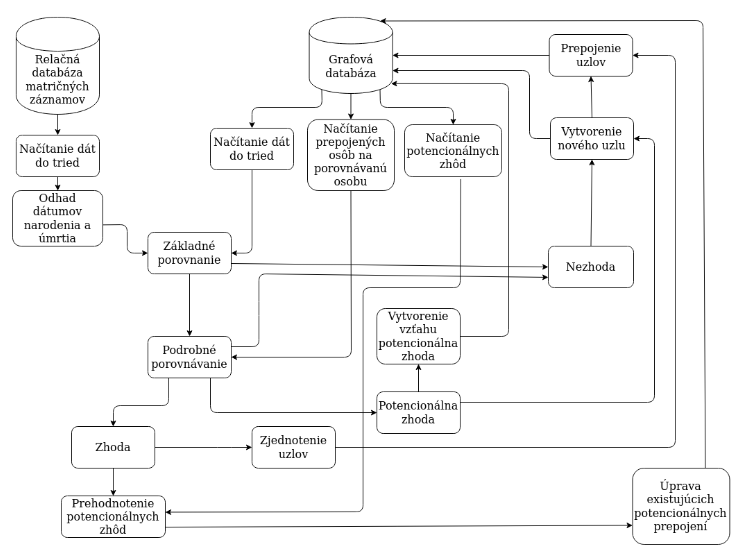
\includegraphics[width=1\textwidth]{obrazky-figures/diagram-original.PNG}
\caption{Návrh celého systému v pôvodnej forme}
\end{figure}

Na obrázku \ref{system} prevzatom zo zdroja \cite{formalniDP} môžeme vidieť celý návrh pôvodného systému. Keďže vieme, že problém je v práci s grafovou databázou, budú sa zmeny musieť týkať hlavne tejto časti. Pokúsime sa teda eliminovať časť neustáleho načítania dát z grafovej databázy, teda úseky \textit{Načítanie dát do tried}, \textit{Načítanie prepojených osôb na porovnávanú osobu} a \textit{Načítanie potencionálnych zhôd}. Jedným z riešení, ktoré som pri vytváraní výsledného návrhu skúmal bolo udržiavať časť dát z grafovej databázy v objektoch jazyku python a minimalizovať tak počet dotazov na databázu. Tým pádom by sme si dáta natiahli iba raz, a pri ukladaní nových osôb do grafovej databázy by sme si tieto osoby pridali aj do spomínaných objektov. Problémom tohoto spôsobu čiastočnej optimalizácie bol však fakt, že pri ukladaní osôb do databázy často dôjde ku zmene vzťahov a aj informácií o osobách, či prípadnému mazaniu a zjednocovaniu osôb. Okrem toho by sa nejednalo o najlepší spôsob optimalizácie z dôvodu, že stále musíme opakovane pristupovať do grafovej databázy, a to nie len pre ukladanie osôb, ale aj pri zjednocovaní uzlov osôb, prepájaní vzťahov, mazaní uzlov osôb alebo aj aktualizácii pri nájdení zhodnej osoby. Pre dosiahnutie najlepšej optimalizácie výsledného systému by sme teda potrebovali okrem neustáleho načítania dát eliminovať aj časť neustáleho vkladanie dát do grafovej databázy. Tu sa ukázalo ako najefektívnejšie riešenie nepracovať s grafovou databázou počas procesu porovnávania vôbec. Všetky dáta, ktoré boli pôvodne držané v grafovej databáze by sme teda potrebovali reprezentovať výhradne pomocou objektov jazyku python. Tu si musíme uvedomiť, že aby sme toto mohli vykonať, bude nutné už existujúce objekty reprezentujúce osoby, záznamy ale aj ďalšie uzly z neo4j podstatne rozšíriť takým spôsobom, aby sme mohli reprezentovať všetky spojenia, ktoré budú existovať vo výslednej databáze v reálnom čase. Bude preto nutné vytvoriť novú triedu pre spravovanie všetkých python objektov držaných výhradne v pamäti a pre vykonávanie operácii nad nimi.

\begin{figure}[h]
\label{after}
\centering
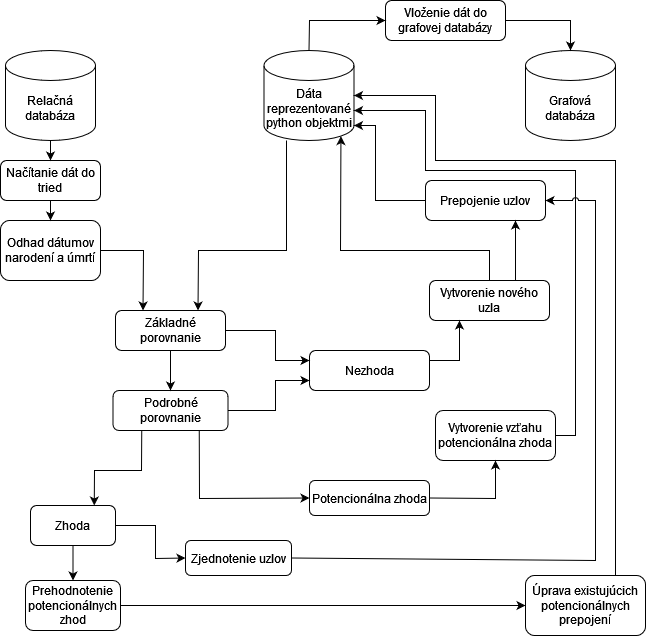
\includegraphics[width=1\textwidth]{obrazky-figures/Untitled Diagram.drawio.png}
\caption{Návrh výsledného systému}
\end{figure}

Z obrázku \ref{after} môžeme vidieť, že v takto zmenenom systéme sa budú dáta držať v pamäti na hromade a budú uložené v python objektoch, odpovedajúcich štruktúre a vzťahom z grafovej databázy. Tým by sme eliminovali proces neustáleho vytvárania a vykonávania dotazov v jazyku cypher nad v istom bode už pomerne objemnou databázou. Na konci porovnávania budú dáta do grafovej databázy vložené naraz až vo výslednej podobe. V takomto prístupe však existuje aj nevýhoda oproti pôvodnej implementácii a to je fakt, že na to, aby sme dostali finálny výstup v podobe grafovej databázy musíme počkať do konca procesu porovnávania a vkladania. Toto však nie je veľmi podstatné, keďže je skript možné jednoducho modifikovať takým spôsobom, aby spracoval iba fixný počet záznamov, napríklad pomocou jednoduchého počítadla v hlavnom cykle (napríklad pri testovacom spúštaní skriptu).

\chapter{Implementácia}

V tejto kapitole sa budeme venovať analýze a oprave chýb a prípadných nedostatkov práce, ďalej si povieme niečo ku implementácii nového prerobeného algoritmu, hlavne pri práci s grafovou databázou, kde dochádza ku výraznému spomaleniu algoritmu. Potom sa pozrieme na presný spôsob implementácie rozšírení týkajúcich sa nových matrík (teda nových typov záznamov o sobáši a úmrtí) vrátane zmien potrebných pri prechode na novú relačnú databázu demos, ktorej štruktúra sa mierne zmenila. Na záver si ukážeme novú formu výstupu vo vyhľadávacích skriptoch a ako boli implementované nové metriky použité pri porovnávaní.

\section{Identifikovanie nedostatkov}

Hľadanie nedostatkov a chýb a ich následné riešenie sa ukázalo byť jedným z najkomplikovanejších a časovo najnáročnejších aspektov tejto práce. Bolo tomu tak najmä kvôli veľkému rozsahu zdrojového kódu skriptov, ale aj kvôli vysokému počtu modulov, ktoré sú navzájom všetky prepojené. Ku odhaleniu chýb došlo najmä pri neustálom spúšťaní skriptu nad rozlyčnými dátami, či už z databázy alebo zo súborov csv, a postupným prechádzaním zdrojového kódu. Často sa ani nejednalo vyslovene o chyby, ale skôr nedostatky, ktoré sa ukázali ako zbytočné, či prípadne o funkcionality, ktoré bolo možné implementovať efektívnejším spôsobom. Väčšina chýb sa týkala práce s grafovou databázou Neo4j a dotazov nadňou, ale niekoľko problémov bolo i v reprezentácii dát a samotnom porovnávaní osôb. V tejto podkapitole si priblížime proces identifikovania chýb a konkrétne chyby a nedostatky, na ktoré som počas vypracovávania práce narazil. Pri každom probléme ukážem aj ako som ho vyriešil.

\subsection{Počiatočné úpravy}

V tejto sekcii si ukážeme ako bolo nutné skript upraviť, aby bol opäť funkčný.

\subsubsection{Identifikovanie problému}

Pred začatím akéhokoľvek implementovania navrhnutých zmien bolo nutné skript najprv upraviť, kedže v stave v akom som ho dostal ho nebolo možné spustiť. Išlo o chybu v module \textit{graph\textunderscore database.py}, pri ktorej sa vo funkcii, ktorá vytvárala dotaz v jazyku cypher, ktorý mal získať všetky adresy osoby z grafovej databázy pristupovalo ku python štruktúre typu slovník na neexistujúci kľúč. Tento slovník mal reprezentovať osobu z grafovej databázy, avšak žiaden kľúč pre ID osoby v slovníku nebol. Dôvodom pre toto mohlo byť, že niektoré zo starších verzií grafovej databázy Neo4j alebo ovládača pre túto databázu v štruktúre typu slovník reprezentujúcej uzol získaný z databázy uvádzali aj ID uzla. Rovnaký problém mali aj niektoré ďalšie funkcie v module s grafovou databázou.

\subsubsection{Riešenie problému}

Keďže ID osoby nebolo v spomínanej funkcii s názvom \textit{get\textunderscore addresses\textunderscore of\textunderscore person\textunderscore from\textunderscore graph\textunderscore db} dostupné, nebolo možné túto querry vytvoriť a spustiť nad databázou. Bolo preto nutné ID osoby nejakým spôsobom získať a propagovať do tejto funkcie. Jednoduchým riešením, ktoré mi napadlo bolo pridať ID samotného uzla ako atribút osoby, tým pádom by sme pri každej osobe získali aj ich ID. Preto som pri vytváraní osôb z grafovej databázy pridal atribút, ktorý sa pri vytvorení uzla nastaví na ID samotného vytváraného uzla.

\subsection{Pohlavia osôb}
Pri určení cieľovej skupiny, s ktorou má daná osoba zo záznamu byť porovnávaná na základe pohlavia dochádzalo pri každej osobe k tomu, že sa porovnávala so všetkými osobami namiesto toho, ako bolo pôvodne zamýšľané (teda iba s osobami rovnakého pohlavia). Zdrojové dáta boli v poriadku a pohlavia osôb boli v databáze i csv súboroch uložené tak, ako mali byť, teda správne označené ako 'M' - muž (male), 'F' alebo 'Ž' - ako žena (alebo female) a pri neidentifikovanom pohlaví ako 'U' - unidentified. Problémom bol spôsob kontroly pohlaví pri spracovávaní osôb. Z dôvodu účelu práce musí každý atribút objektov reprezentujúcich uzly z databázy Neo4j byť uložený ako list. Je tomu tak preto, že niektoré vlastnosti môžu mať v databáze viacero hodnôt a aj kvôli tomu, že pri aktualizácii informácií osoby pri zjednocovaní uzlov osôb si je nutné ponechať všetky informácie, jednak o pôvodnej osobe a aj o osobe, ktorú s ňou zjednocujeme. Pri kontrole pohlavia sa tento fakt však nezohľadňoval a pohlavie sa nesprávne porovnávalo ako objekt typu list, namiesto konkrétnej hodnoty v tomto liste. Tým pádom sa skript vždy vydal do tej istej vetvy a to síce tej, kde pohlavie osoby bolo označené za neidentifikované.
\newline

Riešenie tohoto problému bolo triviálne, preto si ho zhrnieme iba veľmi stručne. Na mieste kontroly pohlaví je pridaná jednoduchá kontrola toho, koľko hodnôt má táto osoba v tomto atribúte. V prípade, že je hodnota jedna, tak pohlavie určíme jednoducho pomocou pristúpenia na túto hodnotu. V prípade že sú v liste dve hodnoty, skontrolujeme, či sú obidve hodnoty iba znaky 'Z' alebo 'F', označujúce ženské pohlavie. V opačnom prípade môžeme prehlásiť, že výsledné pohlavie osoby je nedefinované, kvôli rôznym hodnotám tohoto atribútu. To isté môžeme taktiež prehlásiť, ak sú pohlavia v liste viac ako dve.

\subsection{Porovnávanie osôb spolu s predkami}

Pri analýze kódu som narazil na chybu, ktorá spôsobovala, že predkovia osoby zo záznamu boli porovnávaní s nesprávnym predkom osoby z grafovej databázy. Rola osoby je identifikovaná pomocou reťazca, ktorý je rovnaký ako enumeračný typ určený pre roly osôb z databázy. Šlo o prípad, kedy boli porovnávaní rodičia osoby zo záznamu. Tých reprezentujú roly, ktoré majú v programe názov \textit{f} a \textit{m}. Chyba nastala ak sme chceli porovnávať rodičov rodičov, teda starých rodičov hlavnej osoby zo záznamu. Pri porovnaní predkov osoby je samozrejme žiadúce porovnávať osoby v rovnakom vzťahu ku pôvodnej osobe. Napríklad pri porovnávaní osoby, ktorá má v zázname rolu otcova matka (teda vzťah reprezentovaný ako reťazec \textit{f\textunderscore m}) je žiadúce túto osobu porovnávať s osobou z grafovej databázy, ktorá má ku pôvodnej osobe rovnaký vzťah. Avšak vo funkcii realizujúcej toto porovnanie s názvom \textit{comparison\_of\_two\_person\_with\_ancestors} tomu tak nebolo. Namiesto toho, aby sme osobu vo vzťahu otcova matka porovnávali aj s otcovou matkou zo záznamu, bola osoba z grafovej databázy porovnávaná s osobou s rolou \textit{m\textunderscore f}, teda matkin otec. Rovnako tomu bolo aj v opačnom prípade, teda v prípade porovnania matkinho otca, ktorý bol nesprávne porovnávaný s otcovou matkou. Toto mohlo mať mierny negatívny vplyv na výsledky porovnaní. Oprava chyby spočívala iba v zmenení hodnôt reprezentujúcich rolu osoby na správnu hodnotu.

\subsection{Práca s dátumami}

V tejto podsekcii si povieme, ako sa v pôvodnej implementácii pracovalo s dátumami a ukážeme si, ako sa s nimi bude pracovať po vykonaných zmenách.

\subsubsection{Modul date.py}

Pre prácu s dátumami sa v implementácii používa modul \textit{date.py}. V tomto module sa nachádza trieda \textit{Date}. Jej atribútmi je celý objekt dátumu v podobe objektu typu datetime, rok, mesiac a deň dátumu. Trieda ďalej ponúka viacero funkcií realizujúcich vyžadované operácie nad objektami vytvorenými z tejto triedy, ako napríklad úpravu dátumu pri dni, ktorý je mimo rozsah daného mesiaca, funkciu pre vytvorenie objektu \textit{Date} zo vstupného reťazca či metódu pre výpis dátumu. Pri analýze kódu som došiel ku záveru, že je tento modul zbytočný. Jediná funkcionalita, ktorú ponúka naviac v porovnaní s klasickým python modulom pre reprezentáciu a prácu s dátumami \textit{datetime}, je implementovaná funkcia \textit{change\textunderscore date\textunderscore to\textunderscore nearest\textunderscore possible}. Tá pri dni v mesiaci, ktorý je mimo rozsah daného mesiaca posunie dátum na najbližší ďalší existujúci deň. Avšak implementáciou podobnej funkcie v module \textit{relational\textunderscore database\textunderscore birth.py}, ktorú je nutné aj tak implementovať, kvôli chýbajúcim údajom v dátumoch v novej použitej databáze demos, ktoré bude nutné aj tak nahradiť existujúcou hodnotou. Ďalším dôvodom prečo bolo výhodné tento modul odstrániť bol fakt, že pri prerábaní systému došlo ku viacerým rozsiahlým zmenám a s modulom sa v porovnaní s modulom \textit{datetime} pracuje zbytočne o dosť viac komplikovane, keďže je nutné pre výpis, konverziu či načítanie a uloženie dát volať špeciálne funkcie tohto modulu, nehovoriac o fakte, že modul je v podstate iba komplikovanejší spôsob uchovávania objektu triedy \textit{datetime.datetime} s dodatočnými krokmi.

\subsubsection{Odstránenie modulu}

Modul som sa rozhodol z implementácie odstrániť úplne a namiesto objektov, ktoré implementuje trieda \textit{Date} som sa rozhodol pre reprezentovanie a prácu s dátumami použiť existujúci modul \textit{datetime}, ktorý ponúka triedu \textit{datetime.datetime}. Ten je pre reprezentáciu dátumov ideálny a ponúka všetky potrebné funkcionality implementované pôvodným modulom, ako funkcie \textit{strptime} a \textit{strftime}, ktoré umožnujú jednoducho konvertovať reťazce na \textit{datetime.datetime} objekty a naopak.

\subsubsection{Nutné zmeny po odstránení}

Po odstránení modulu bolo nutné vykonať viacero zmien. Išlo o zmeny pri určovaní dátumov podľa rôl osôb, načítaní dát a v podstate na každom mieste v kóde, kde dochádzalo ku porovnaniam medzi dátumami a prevodom z reťazca na typ reprezentujúci dátum a naopak. V module \textit{relational\textunderscore database\textunderscore birth.py} bolo nutné potom implementovať požadovanú funkcionalitu zmenenia neexistujúcich dátumov na existujúce a to pomocou funkcie \textit{replace\textunderscore double\textunderscore questionmarks}, ktorá vykonáva doplnenie chýbajúcich dát takým spôsobom, že v prípade chýbajúceho dňa a mesiaca je deň alebo mesiac nastavený na prvý deň v mesiaci alebo teda prvý mesiac v roku. Funkcia zohľadňuje aj počet dní, ak vieme o aký mesiac sa jedná a naopak, ak by bol deň mimo rozsah mesiaca, vyberie iba odpovedajúce mesiace, ktoré môžu daný počet dní mať. Okrem funkcie sú na mieste spracovania dátumov aj ďalšie kontroly, či napríklad nedošlo ku zameneniu údaju o dni s údajom o mesiaci. Toto môžeme prehlásiť, ak je údaj dňa menší ako 12 a údaj o mesiaci väčší ako 12. V takomto prípade sa predpokladá zamenenie hodnôt a hodnoty údajov sú vymenené.

\subsection{Mazanie databázy}

V tejto sekcii si priblížime problém, ktorý vznikol pri mazaní databázy, ktorá bola naplnená vysokým objemom dát.

\subsubsection{Identifikovanie problému s mazaním}

Počas testovania nad databázou som narazil na problém, ku ktorému dochádzalo pri snahe zmazať celú databázu pri novom spustení skriptu. Keďže Neo4j community edition neponúka možnosť databázu zmazať pomocou drop dotazu (funkcionalita je dostupná iba pre Neo4j enterprise edition), bola databáza mazaná vytvorením dotazu odpovedajúcemu všetkým prvkom databázy a následnému zmazaniu všetkých vzťahov a uzlov.

\begin{figure}[h]
\label{deletion}
\begin{lstlisting}[language=SPARQL]
                            MATCH (n) DETACH DELETE n
\end{lstlisting}
\caption{Dotaz používaný na mazanie databázy}
\end{figure}

Na obrázku \ref{deletion} môžeme vidieť dotaz realizujúci mazanie v pôvodnej implementácii. Problém nastáva vtedy, keď je v databáze veľký objem dát a z tohto dôvodu pri snahe o vytvorenie takéhoto dotazu dôjde ku chybe typu java heap error. To znamená, že pri snahe pomocou dotazu označiť príliš veľké množstvo dát dôjde jazyku java, v ktorom je databáza Neo4j implementovaná pamäť na hromade.

\subsubsection{Možné riešenia}

Na vyriešenie tohoto problému sa ponúkalo viacero spôsobov. Prvým by bolo zo skriptu za použitia python modulu s názvom \textit{os} manuálne pristúpiť a zmazať zdrojové súbory databázy. Avšak problémom tohto riešenia je, že skript by potom musel byť vždy spúšťaný s administrátorskými právami, čo nie je veľmi praktické. Taktiež by vznikol problém pri zisťovaní cesty k týmto súborom, keďže databáza Neo4j môže byť nainštalovaná na rôznych miestach a súbory s databázou môžu mať podľa platformy, na ktorej je databáza nainštalovaná rôzne umiestnenie. Toto riešenie preto nie je veľmi vhodné. Ďalšou možnosťou by bolo manuálne zvýšenie množstva pamäťe na hromade, ktoré java priraďuje aplikácii Neo4j. Avšak tu sa nejedná o úplné riešenie problému, ale skôr iba o odsunutie. Potom by tu bola možnosť prechodu z Neo4j Community Edition na Neo4j Enterprise Edition. Táto edícia databázy je však platená a kvôli jedinej požadovanej funkcionalite by to bolo zbytočné. Najlepším riešením sa ukázalo byť mazanie databázy v menších dávkach (tzv. batch deletion). To ale nie je možné vykonať pomocou jediného dotazu. Bolo preto nutné pridať jednoduchý algoritmus realizujúci opakované cypher dotazy dovtedy kým databáza nie je prázdna.

\begin{figure}[h]
\label{batchdelete}
\centering
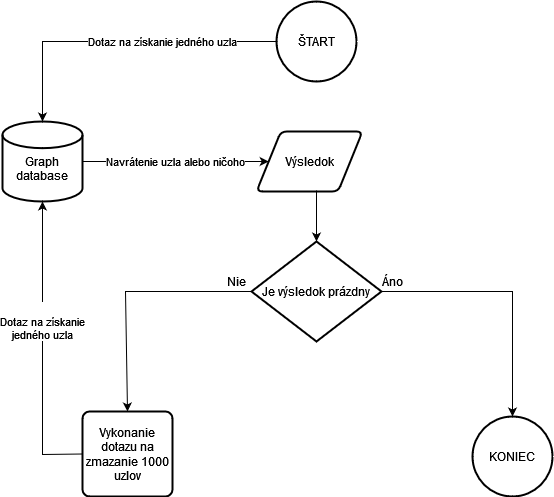
\includegraphics[width=0.8\textwidth]{obrazky-figures/Database-deletion.png}
\caption{Schéma algoritmu mazania}
\end{figure}

Na obrázku \ref{batchdelete} môžeme vidieť algoritmus mazania databázy. Na začiatku sa vykoná jednoduchý dotaz na získanie jediného uzla. Vo výsledku dotazu následne skontrolujem, či nie je prázdny. V prípade, že je výsledok prázdny môžeme prehlásiť databázu za prázdnu a teda pokračovať vo vykonávaní samotného skriptu. V prípade, že výsledok dotazu nie je prázdny, vykonáme dotaz na zmazanie tisícich uzlov z databázy. Ďalej pokračujeme rovnakým dotazom na získanie jediného uzla z databázy a proces sa takto opakuje, až kým databáza nie je prázdna.

\subsection{Ďalšie optimalizácie}

V skripte bolo vykonaných množstvo ďalších menších optimalizácií, ktoré samé o sebe veľmi nestoja za zmienku. Išlo najmä o odstránenie zbytočných funkcií realizujúcich triviálne operácie. Jedná sa o funkcie, ktoré mohli byť napríklad nahradené jednou podmienkou, alebo realizujúcich minimálne množstvo kódu, teda iba pridávali extra réžiu spôsobenú svojím volaním. Ďalšou optimalizáciou, ktorá možno stojí za zmienku je nahradenie neustálého používania operátora \textit{+} jazyka python pre konkatenáciu reťazcov. Ten môže byť pri konkatenácii väčšieho množstva reťazcov výrazne menej efektívny ako metóda \textit{join} z modulu \textit{string}. Tá môže byť podľa informácií zo zdroja \cite{plusop} až 4-krát efektívnejšia pri konkatenácii viacerých reťazcov ako operátor \textit{+}. Takéto optimalizácie nemusia mať pri spracovávaní menšieho množstva dát veľmi výrazný efekt, ale pri spracovávaní veľkého objemu dát sa už môže jednať o signifikantné množstvo ušetreného času, hlavne ak si uvedomíme, že počas behu skriptu dochádza ku konkatenácii reťazcov pomerne často.

\subsection{Skript get\_all\_records.py}

Tento skript bol v pôvodnom stave implementácie nefunkčný. Pri získavaní dát o úlohe osoby v špecifickom zázname a pri získavaní dátumu záznamu sa ku navrátenej štruktúre s týmito údajmi pristupovalo nesprávne. Tento problém bol jednoducho vyriešiteľný úpravou spôsobu, akým sa k týmto dátam pristupuje.

\section{Implementácia zmeneného systému}

V tejto podkapitole si povieme ako prebiehala a čo všetko zahŕňala implementácia nového navrhnutého systému. Postupne si prejdeme jednotlivé zmeny, ktoré táto optimalizačná zmena priniesla.

\subsection{Rozbor problematiky}

Hlavným riadiacim bodom celého algoritmu je modul \textit{create\_database.py}. Ten riadi celý proces porovnávania a spracovávania dát. Celý proces pozostáva z načítania dát z relačnej databázy pomocou metód z triedy \textit{RelationalDatabaseHandle}, ktorá je implementovaná v module \textit{relational\_database\_birth.py}, následnému načítania všetkých osôb z grafovej databázy pomocou metód z triedy \textit{GraphDatabaseHandle}, ktorá je implementovaná v module \textit{graph\_database.py} a ich následnému porovnávaniu pomocou funkcií z modulu \textit{comparator.py}. Počas celého procesu sa celý čas pracuje priamo nad grafovou databázou. To znamená, že ak napríklad klasifikujeme osobu ako nezhodu a chceme ju vložiť do databázy, musíme hneď zavolať metódu triedy \textit{GraphDatabaseHandle}, ktorá vytvorí a vykoná dotaz priamo nad databázou v reálnom čase. Týmto sa pri každej spracovávanej osobe zakaždým mení štruktúra grafovej databázy, preto je nutné ju po každom spracovanom zázname celú znova načítať aj s jej novou štruktúrou pomocou dotazov v jazyku Cypher. Takýto algoritmus je pomerne časovo náročný a neefektívny.
\newline

Keďže už vieme, ako by mal výsledný optimalizovaný systém vyzerať, ukážeme si ako sa bude celý algoritmus meniť. Vieme už, že dáta nechceme zakaždým ukladať priamo do databázy a opakovane ju celú za každým záznamom znova načítať. Preto musí existovať nejaká medzivrstva, ktorá dokáže reprezentovať dáta vkladané do grafovej databázy Neo4j, teda spôsob ako reprezentovať štruktúru dát uložených v tejto databáze. V implementácii tejto medzivrstvy bude nutné reprezentovať teda nie len samotné uzly, ale aj všetky vzťahy ktoré sú medzi nimi.

\subsection{Reprezentácia dát}

Keďže potrebujeme reprezentovať veľké množstvo rôznych uzlov, ktoré majú medzi sebou rôzne typy vzťahov, bude nutné vybrať čo najuniverzálnejší spôsob reprezentácie dát, ktorý bude fungovať pre všetky typy uzlov a vzťahov. V implementácii už existujú triedy, ktoré reprezentujú jednotlivé uzly z databázy Neo4j. Avšak zatiaľ medzi nimi nie je žiaden spôsob reprezentácie vzťahov. Jedná sa o triedy \textit{Person}, \textit{Record} a \textit{Register}. Pre reprezentovanie uzlov adries, teda miest, ulíc a popisných čísel je použitá trieda \textit{Domicile}, ktorá slúži skôr na implementáciu ukladania adries osôb, nie samotných miest, ulíc, popisných čísel a vzťahov medzi nimi. Jedná sa teda skôr o spôsob ako uchovať informáciu o adrese osoby a nie celkovú štruktúru mesta, na ktoré sú prepojené ulice, na ktoré sú následne prepojené všetky popisné čísla v ulici. Toto je v pôvodnej implementácii implementované neustálým kontrolovaním existencie duplicitných uzlov opäť priamo nad databázou.

\begin{figure}[h]
    \centering
    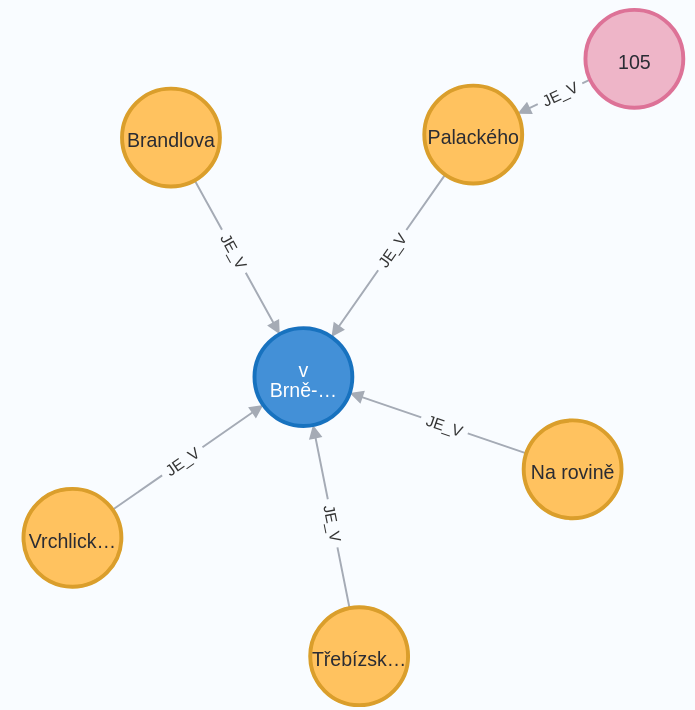
\includegraphics[width=0.8\textwidth]{obrazky-figures/adresses.png}
    \caption{Ukážka štruktúry uzlov adries}
    \label{adress}
\end{figure}

Na obrázku \ref{adress} môžeme vidieť jednoduchý demonštračný príklad. Modrý uzol reprezentuje mesto alebo dedinu, oranžový uzol ulicu a ružový uzol popisné číslo. Uzly sú následne hierarchicky prepojené podľa príslušnosti vzťahom \textit{JE\_V}. Ak by sme v databáze mali uloženú nasledujúcu štruktúru dát mesta a adries v ňom a pri spracovávaní osoby by sme sa dostali ku adrese osoby (objekt typu \textit{Domicile}), musel by byť opäť vykonaný dotaz nad databázou, aby sme zistili, či takáto adresa už v databáze existuje a následne v prípade, že už existuje, osobu prepojiť na túto adresu. V opačnom prípade by musel byť ešte aj vytvorený nový uzol pre novú adresu, opäť v reálnom čase nad databázou.

\subsubsection{Pridanie modulu data\_representation.py}

Pridávanie reprezentácie vzťahov a všetkých uzlov vo výslednej databáze si rozoberieme hierarchicky, to znamená, že začneme uzlom záznamu, ktorý nesie aj informáciu o matrike z ktorej pochádza, následne si prejdeme reprezentáciu osôb a na záver si ukážeme ako budú reprezentované uzly adries. Ešte predtým si musíme vytvoriť jednoduchý spôsob prístupu ku všetkým objektom a ich vzťahom. Preto som vytvoril nový modul implementujúci triedu \textit{DataRepresentation}. Tá bude tvoriť už spomínanú medzivrstvu pred ukladaním dát do grafovej databázy. Bude obsahovať objekty reprezentujúce všetky uzly, ich vzťahy a všetky potrebné metódy pre operácie, ktoré bude nutné vykonávať nad touto vzniknutou štruktúrou. V module \textit{create\_database.py} si potom iba vytvoríme novú inštanciu tohoto objektu a tak budeme môcť jednoducho pristupovať ku všetkým dátam a metódam. Dá sa povedať, že tento modul implementuje funkcionality, ktoré boli vykonávané v module \textit{graph\_database.py} priamo nad databázou, ale vykonáva ich nad navrhnutou reprezentáciou dát.

\subsubsection{Reprezentácia dát pomocou objektov}

Keďže potrebujeme reprezentovať veľké množstvo uzlov, bude najvhodnejšie uchovávať ich v objekte typu list z jazyku python. Takto môžeme vyriešiť ukladanie samotných objektov. Spôsob ukladania jednotlivých vzťahov sa bude pri každom type vzťahov trochu líšiť preto si o nich povieme, až keď sa dostaneme ku danému vzťahu. Objekty budú teda uložené ako atribúty v novej vzniknutej triede \textit{DataRepresentation} a budú mať formu listu. Ak teda začneme hierarchycky samotnými záznamami, tie sú reprezentované objektom \textit{Record}. Preto bude vhodné vytvoriť list všetkých objektov záznamov. Pri kažom spracovávanom zázname si teda daný záznam uložíme do tohto listu. Ďalej nasleduje objekt reprezentujúci matriku. Tým je objekt implementovaný triedou \textit{Register}. Tu budeme opakovať rovnaký postup a opäť vytvoríme list všetkých týchto objektov. Tak ako v pôvodnej implementácii bude ale nutné kontrolovať, či sa už matrika záznamu v liste nenachádza. Špeciálnu reprezentáciu vzťahu, ktorý medzi sebou má matrika a záznam matriky teda už nemusíme pridávať, keďže záznam má ako jeden zo svojich atribútov ID matriky, z ktorej pochádza. Preto ho budeme vedieť vo výsledku jednoducho prepojiť na správnu matriku z listu matrík. Príklad štruktúry databázy, ktorú sme takto práve implementovali môžeme vidieť na obrázku \ref{matrika}. Na ňom môžeme vidieť hnedý uzol reprezentujúci matriku a červené uzly reprezentujúce záznamy z matriky, ktoré sú na matriku prepojené vzťahom \textit{JE\_V}.

\begin{figure}[H]
    \centering
    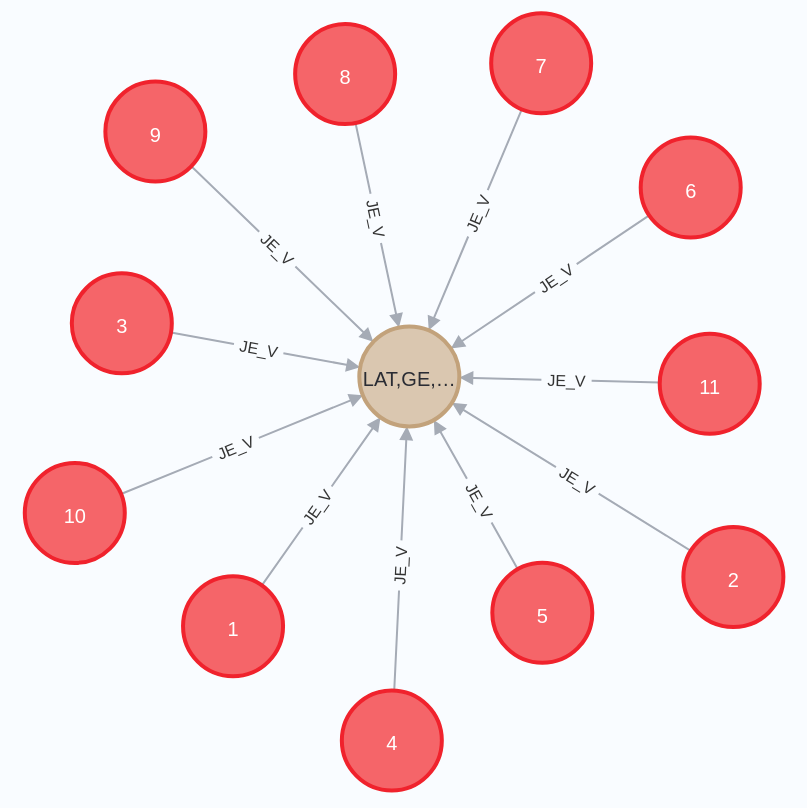
\includegraphics[width=0.8\textwidth]{obrazky-figures/matrika.png}
    \caption{Výsledná štruktúra záznamov prepojených na matriku}
    \label{matrika}
\end{figure}

Najnáročnejšou časťou bolo implementovať reprezentáciu prepojení osôb s inými osobami a osôb so záznamami. Pre reprezentovanie vzťahov osôb som sa rozhodol vytvoriť nové atribúty objektu \textit{Person}. Tento objekt po novom obsahuje atribút vo forme listu pre reprezentovanie všetkých vzťahov vedúcich z osoby (či už na iné osoby alebo na záznamy) okrem vzťahov potencionálnych zhôd, ktoré sú uložené v osobitnom liste. Okrem toho bolo nutné vedieť aj všetky vzťahy vedúce do uzla osoby, preto som vytvoril ďalší atribút typu list, ktorý uchováva aj tieto vzťahy.

Ďalšími uzlami a vzťahmi, ktoré bolo nutné uchovať sú mestá, ulice a popisné čísla. Pri spracovávaní osoby máme v už spomínanom objekte \textit{Domicile} informácie o adrese osoby. Bude preto nutné na základe informácií obsiahnutých v tomto objekte vytvárať novú štruktúru. Opäť bude vhodné pre uchovanie všetkých objektov miest vytvoriť v triede \textit{DataRepresentation} atribút typu list, do ktorého budú všetky objekty miest ukladané. 

\subsection{Štruktúra pre reprezentovanie vzťahov}

Teraz keď už vieme, kde si budeme vzťahy uchovávať, je nutné navrhnúť štruktúru pre reprezentovanie každého typu vzťahu. Toto budú štruktúry uložené v spomínaných listoch. Ako najlepší spôsob pre reprezentáciu vzťahu sa ukázal byť python objekt typu slovník. Ten uchováva dáta v pároch formou kľúčov, ku ktorým prislúchajú hodnoty.
Takým spôsobom si môžeme uchovať všetky atribúty vzťahov a zároveň reprezentovať smer vzťahov a aj sa odkazovať na uzol na ktorý vzťah smeruje. Smer vzťahov je implicitne vždy smerujúci z uzla okrem prípadu už spomínaného listu s všetkými vzťahmi smerujúcimi do uzla. Pre určenie uzla, s ktorým je pôvodný uzol (reprezentovaný objektom) vo vzťahu, používame referenciu na objekt reprezentujúci cieľový uzol. To v praxi v podstate znamená jednoduché priradenie objektu, keďže v jazyku python je priraďovanie každej hodnoty iba vytvorenie premennej odkazujúcej na rovnaký objekt.

\subsubsection{Vzťahy medzi osobami}

Na obrázku \ref{relationship} môžeme vidieť príklad vzniknutého vzťahu osoby. V tomto prípade sa jedná o vzťah medzi dvoma osobami. Slovník tvoriaci takýto vzťah sa skladá z dvoch kľúčov. Tými sú \textit{type}, ktorého hodnotou je názov vzťahu, ktorý budeme vkladať do databázy, v tomto konkrétnom príklade je to vzťah \textit{JE\_OTEC}. Ďalším kľúčom je \textit{person}, ktorého hodnotou je už samotný odkaz na objekt reprezentujúci cieľový uzol, v tomto prípade by išlo o dieťa osoby. Zakaždým, keď vytvárame takýto vzťah, je vytvorený aj vzťah v liste vzťahov smerujúcich do uzla osoby v atribúte objektu reprezentujúceho cieľový uzol. Takýto vzťah bude mať rovnakú hodnotu kľúča \textit{type} a hodnotou kľúča \textit{person} bude osoba, z ktorej vzťah smeruje. Pre uloženie vzťahov potencionálnych zhôd je potom použitý osobitný atribút. Pri reprezentácii vzťahov je v prípade potencionálnej zhody prítomný aj kľúč s porovnávacím skóre osôb.

\begin{figure}[H]
    \centering
    \begin{lstlisting}[language=python]
                        {
                          "type": "JE_OTEC",
                          "person": person_variable
                        }              
    \end{lstlisting}
    \caption{Slovník reprezentujúci vzťah osoby s inou osobou}
    \label{relationship}
\end{figure}

\subsubsection{Vzťah medzi osobou a záznamom}

Ďalším typom vzťahov, ktoré môže osoba mať sú vzťahy ku záznamom. V týchto vzťahoch potrebujeme ukladať opäť typ vzťahu, objekt na ktorý sa vzťahom odkazujeme a k tomu ešte aj dátum vytvorenia záznamu. Na obrázku \ref{relationship-record} môžeme vidieť štruktúru slovníka reprezentujúceho takýto vzťah. Opäť je tu kľúč \textit{type}, ktorého hodnotou je názov vzťahu. Ďalej tu máme kľúč \textit{record}, ktorého hodnota je odkaz na samotný objekt reprezentujúci záznam. Potom je tu ešte kľúč \textit{date}, ktorého hodnota je objekt triedy \textit{datetime.datetime} reprezentujúci dátum záznamu.

\begin{figure}[H]
    \centering
    \begin{lstlisting}[language=python]
                        {
                          "type": "OTEC",
                          "record": record_variable,
                          "date": date
                        }              
    \end{lstlisting}
    \caption{Slovník reprezentujúci vzťah osoby so záznamom}
    \label{relationship-record}
\end{figure}
\pagebreak

Na obrázku \ref{people} môžeme vidieť, akú štruktúru dát sme vytvorenými vzťahmi dokázali reprezentovať. Ide o príklad záznamu o krste a všetkých osôb, ktoré v ňom figurujú vrátane všetkých vzťahov medzi osobami a osobami a záznamom. Červený uzol tu reprezentuje záznam o krste a zelené uzly reprezentujú osoby figurujúce v zázname.

\begin{figure}[H]
    \centering
    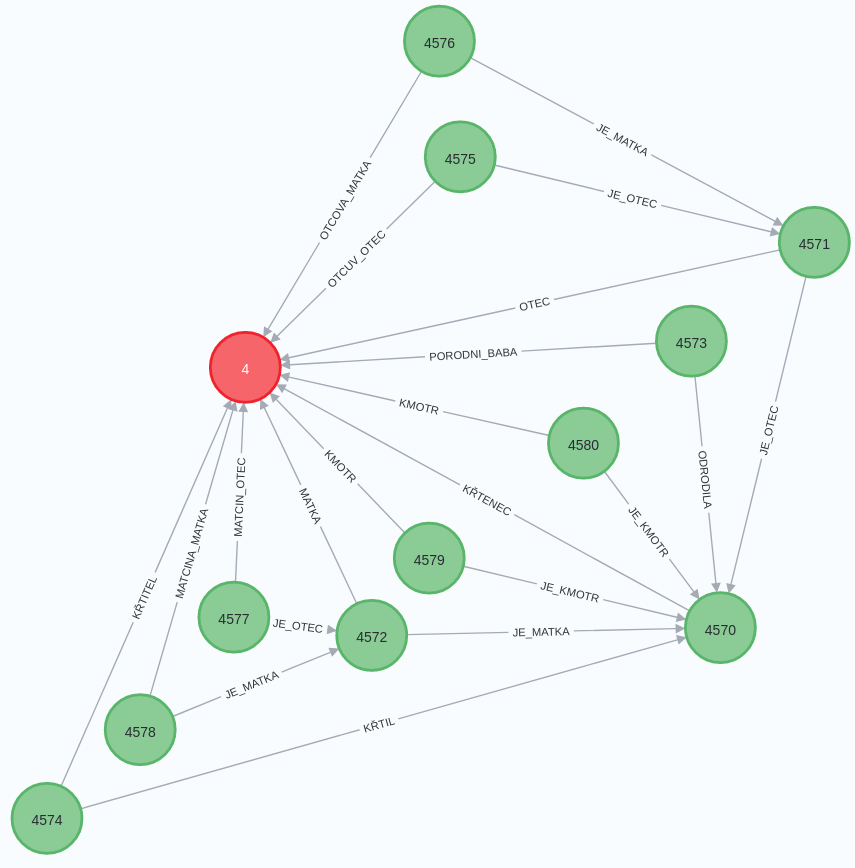
\includegraphics[width=0.8\textwidth]{obrazky-figures/people.png}
    \caption{Príklad osôb a ich vzťahov v databáze}
    \label{people}
\end{figure}

\subsubsection{Vzťah medzi osobou a uzlom adresy}

Tento typ vzťahu nebolo nutné reprezentovať novou štruktúrou, keďže každý objekt \textit{Person} už má atribút typu list objektov typu \textit{Domicile}, ktorý nám hovorí na akých adresách osoba počas života bývala. Jediné čo bolo nutné v tomto atribúte modifikovať bolo pridanie špecifického ID k atribútu ulice a popisného čísla. Toto bolo vykonané z implementačných dôvodov pri vytváraní štruktúr reprezentujúcich hierarchiu vzťahov medzi uzlami adries (teda mestami, ulicami a popisnými číslami). Keďže sme prestali robiť neustále dotazy na adresy v databáze, stratili sme informácie o existujúcich mestách a ulicách a popisných číslach v nich. To ako sme si tieto vzťahy reprezentovali si popíšeme v ďalšej sekcii. Vzťahy osôb k najdetailnejšiemu uzlu adresy (teda vzťahy \textit{BÝVA}) si vieme prepojiť jednoducho podľa atribútu s adresami osoby.

\subsection{Hierarchia vzťahov uzlov adries}

Ako už vieme, adresy uložené v databáze majú vlastnú hierarchiu vytvorenú na základe príslušnosti ulíc mestám a popisných čísel uliciam, či prípadne dedinám. Keďže sú všetky mestá uložené v liste v atribúte triedy \textit{DataRepresentation} bolo ideálne ukladať celú hierarchiu týchto vzťahov do štruktúry reprezentujúcej mesto. Najlepšou štruktúrou pre uloženie mesta a jeho vzťahov sa opäť ukázal byť slovník, keďže potrebujeme ukladať viacero pomenovaných údajov s ich hodnotami a zároveň aj vzťahy mesta (teda ulice a popisné čísla prepojené na mesto).

\lstset{
    inputencoding=utf8,
    extendedchars=true,
    literate=%
    {á}{{\'a}}1
    {č}{{\v{c}}}1
    {ď}{{\v{d}}}1
    {é}{{\'e}}1
    {ě}{{\v{e}}}1
    {í}{{\'i}}1
    {ň}{{\v{n}}}1
    {ó}{{\'o}}1
    {ř}{{\v{r}}}1
    {š}{{\v{s}}}1
    {ť}{{\v{t}}}1
    {ú}{{\'u}}1
    {ů}{{\r{u}}}1
    {ý}{{\'y}}1
    {ž}{{\v{z}}}1
    {Á}{{\'A}}1
    {Č}{{\v{C}}}1
    {Ď}{{\v{D}}}1
    {É}{{\'E}}1
    {Ě}{{\v{E}}}1
    {Í}{{\'I}}1
    {Ň}{{\v{N}}}1
    {Ó}{{\'O}}1
    {Ř}{{\v{R}}}1
    {Š}{{\v{S}}}1
    {Ť}{{\v{T}}}1
    {Ú}{{\'U}}1
    {Ů}{{\r{U}}}1
    {Ý}{{\'Y}}1
    {Ž}{{\v{Z}}}1
}

\begin{figure}[H]
    \centering
    \begin{lstlisting}[language=python]
{
  "id": uuid.uuid4(),
  "name": "V Brně-Husovicích",
  "normalized_name": None,
  "gps": [0.0,0.0]
  "streets": [
		{
		  "street_name": ("Palackého", uuid.uuid4()),
		  "numbers": [
			     	("105", uuid.uuid4())
			      ]
		},
		{
		  "street_name": ("Na rovině", uuid.uuid4()),
		  "numbers": []
		},
		{
		  "street_name": ("Brandlova", uuid.uuid4()),
		  "numbers": []
		},
		{
		  "street_name": ("Třebízského", uuid.uuid4()),
		  "numbers": []
		},
		{
		  "street_name": ("Vrchlického", uuid.uuid4()),
		  "numbers": []
		}
	     ],
  "numbers": []
}
    \end{lstlisting}
    \caption{Príklad slovníka reprezentujúceho mesto a jeho ulice a popisné čísla}
    \label{townstruct}
\end{figure}

Na obrázku \ref{townstruct} môžeme vidieť vzniknutú štruktúru mesta, ktorá reprezentuje všetky uzly a vzťahy, ktoré môžeme vidieť na obrázku \ref{adress}. Mesto je teda reprezentované slovníkom, ktorého kľúče \textit{id}, \textit{name}, \textit{normalized\_name} reprezentujú ID mesta, jeho názov a aj jeho normalizovaný názov v tomto poradí, následne je tu kľúč \textit{gps}, ktorý reprezentuje gps súradnice mesta (v prípade, že sme nenašli hodnotu súradníc získavanú zo súborov JSON, je predvolená hodnota [0.0,0.0]), kľúč \textit{streets}, ktorého hodnotou je list slovníkov reprezentujúcich ulice mesta a posledným kľúčom slovníka mesta je kľúč \textit{numbers}, ktorého hodnotou je zasa list všetkých objektov typu tuple, reprezentujúcich jednotlivé popisné čísla v meste (v prípade, že by sa jednalo o dedinu, alebo v prípade, že by chýbal údaj o ulici, do ktorej popisné číslo patrí).

Pri štruktúre reprezentujúcej ulicu sa jedná opäť o slovník, ktorého kľúče sú \textit{street\_name} a \textit{numbers}. Ich hodnotou je objekt typu tuple jednoznačne identifikujúci ulicu a list objektov typu tuple reprezentujúcich popisné čísla v tomto poradí. Objekt typu tuple reprezentujúci ulicu sa skladá z názvu ulice vo forme reťazca a z ID ulice, ktoré jednoznačne ulicu identifikuje. Pri objekte typu tuple reprezentujúcom popisné čísla ide o presne rovnaký formát dát, číže popisné číslo vo forme reťazca a id. Pre vytvorenie hodnôt ID bola použitá funkcia modulu \textit{uuid}, \textit{uuid4()}, ktorá vygeneruje náhodné ID.

\subsubsection{Vytváranie štruktúry}

Štruktúra miest v takejto podobe vzniká pri spracovaní adries spracovávanej osoby. Pre každú adresu z listu adries osoby je zavolaná funkcia \textit{create\_domicile} modulu \textit{DataRepresentation}. Tá prejde list miest a skontroluje, či sa v ňom nová adresa už nenachádza, pričom kontrola začína zhora nadol, najprv sa kontroluje, existencia mesta, potom ulíc v ňom a nakoniec aj popisných čísel. Vždy sa pridá iba potrebný najdetailnejší údaj, takže nevytvárame žiadne duplicitné mestá ani ulice.

\subsection{Výsledný algoritmus}

Vytvorenie novej podoby algoritmu ktorú som navrhol teda pozostávalo z implementácie modulu \textit{data\_representation.py} vrátane všetkých jeho metód a atribútov v podobe už spomínaných štruktúr, nahradenia všetkých volaní funkcií modulu \textit{graph\_database.py} volaniami funkcií modulu \textit{data\_representation.py}, vykonávajúcich ekvivalentné operácia nad mnou navrhnutými datovými štruktúrami a následným vložením celej výslednej štruktúry uloženej v objektoch do grafovej databázy Neo4j. Týmto spôsobom sme eliminovali a nahradili všetky časti pôvodného algoritmu, ktoré sme si vytýčili v jeho návrhu.


\section{Nové formy vstupných dát}

V tejto podkapitole si rozoberieme proces pridávania nových vstupných dát v podobe matrík úmrtí a matrík sobášov. Pozrieme sa na jednotlivé časti algoritmu, ktoré museli byť modifikované a na nové funkcionality, ktoré museli byť implementované.

\subsection{Úpravy pri zmene relačnej databázy}

Ešte pred začiatkom pridávania podpory pre nové vstupné dáta bolo nutné zmeniť spôsob, akým sa z databázy načítavajú dátumy. V pôvodnej databáze perun nebolo nutné prevádzať dátumy z reťazcov na \textit{datetime.datetime} objekty. Túto konverziu bolo nutné pridať pri každom načítanom dátume do modulu zodpovedného za načítanie dát, teda \textit{relational\_database\_birth.py}. Taktiež formát dátumov v databáze bol často nekonzistentný, s chýbajúcimi údajmi o mesiacoch či dňoch a niekedy aj rokoch. Často sa v hodnotách vyskytovali neexistujúce dni v mesiaci ako napríklad 31.9 alebo 30.2. To vždy spôsobovalo spadnutie programu pri konverzii takéhoto reťazca na objekt typu \textit{datetime.datetime}, ktorý takéto chybné údaje nepodporuje. Na miesto som preto implementoval kontroly, ktoré prípadné chýbajúce údaje doplnia reálnymi datami. Chýbajúci deň v mesiaci je preto nastavený na prvý deň v mesiaci a chýbajúci mesiac zasa na prvý mesiac v roku. Taktiež je na mieste kontrola, či údaje o mesiaci a dni nie sú zamenené. V takom prípade sú vymenené. V budúcnosti by som odporučil vykonať opravu dát v databáze, prmárne dátumov, tak aby tam boli iba reálne a úplné hodnoty, keďze nesprávne hodnoty môžu viesť ku nekonzistenciám.

\subsection{Načítanie dát}

Do modulu načítavajúceho dáta z relačnej databázy \textit{relational\_database\_birth.py} bolo nutné pridať funkcie vykonávajúce načítanie dát z tabuliek záznamov o úmrtí a sobášov, načítanie všetkých osôb figurujúcich v danom zázname a vyplnením novovzniknutých objektov typu \textit{record} a \textit{Person} všetkými údjami získanými z databázy. Taktiež bolo nutné pridať nové funkcie pre získanie dátumu záznamu, keďže dátumy záznamov rozličného typu mali rozličné názvy stĺpcov v ktorých bol dátum uložený a v prípade chýbajúceho záznamu bolo nutné dátum získať implicitne z príslušného odpovedajúceho dátumu z tabuľky osoby, ktorá zastupovala v zázname hlavnú rolu. Objekty \textit{Person} museli byť taktiež rozšírené o nové atribúty, ktorými boli údaje v nových záznamoch. Boli nimi napríklad dátum viatika, pohrebu, sobášu, rozvodu, fakt či dieťa nebolo mrtvorodené a príčina smrti osoby.

\subsection{Odhady dátumov}

Ďalšie zmeny bolo nutné implementovať vo funkcii vykonávajúcej odhad intervalu dátumu narodenia a úmrtia osoby. Tam boli pridané nové odhady vďaka novým typom dátumov a novým rolám osôb a taktiež kontextu udaného typom záznamu. Pri určovaní odhadov bolo nutné ku existujúcim pravidlám pridať nasledujúce pravidlá.

\begin{itemize}
    \item Dátum viatika musel byť najskôr mesiac pred úmrtím osoby
    \item Dátum pohrebu musel byť najneskôr mesiac po úmrtí osoby
    \item Vek matky ženícha alebo nevesty musel byť minimálne 30 rokov a maximálne 60 rokov
    \item Vek otca ženícha alebo nevesty musel byť minimálne 30 rokov a maximálne 70 rokov
    \item Vek starých rodičov ženícha alebo nevesty musel byť minimálne 45 rokov a maximálne 85 rokov
\end{itemize}


\subsection{Modifikácia riadiaceho algoritmu}

Hlavný algoritmus riadiaci porovnávanie a načítanie záznamov bol modifiovaný tak, aby po skončení spracovávania záznamov jedného typu pokračoval záznamami ďalšieho typu. Zároveň po skončení spracovávania jedného záznamu bola pridaná kontrola na typ záznamu, podľa ktorej sa určí aká funkcia na prepojenie osôb zo záznamu bude zavolaná. Bolo teda nutné implementovať aj tieto nové funkcie, ktoré prejdú všetkými osobami záznamu a vytvoria všetky spojenia medzi osobami a záznamami, pomocou metód implementovaných v module \textit{DataRepresentation}. Nové typy záznamov pridali pomerne veľké množstvo nových rôl osôb. Nové roly pridané záznamami úmrtí sú nasledovné.
\pagebreak
\begin{multicols}{2}
\begin{itemize}
    \item ZESNULÝ
    \item SYN\_ZESNULÉHO
    \item DCERA\_ZESNULÉHO
    \item MANŽEL\_ZESNULÉHO
    \item MANŽELKA\_ZESNULÉHO
    \item POCHOVAL
    \item HROBNÍK
    \item ZAOPATŘIL
    \item ZAOPATŘOVATEL
\end{itemize}
\end{multicols}

A nakoniec roly pridané záznamami o sobášoch sú nasledovné:
\begin{multicols}{2}
    \begin{itemize}
        \item ŽENÍCH
        \item JE\_MANŽEL
        \item NEVĚSTA
        \item JE\_MANŽELKA
        \item ŽENICHUV\_OTEC
        \item ŽENICHOVA\_MATKA
        \item NEVĚSTIN\_OTEC
        \item NEVĚSTINA\_MATKA
        \item MATKA\_ŽENICHOVA\_OTCE
        \item OTEC\_ŽENICHOVA\_OTCE
        \item MATKA\_ŽENICHOVY\_MATKY
        \item OTEC\_ŽENICHOVY\_MATKY
        \item MATKA\_NEVĚSTINA\_OTCE
        \item OTEC\_NEVĚSTINA\_OTCE
        \item MATKA\_NEVĚSTINY\_MATKY
        \item OTEC\_NEVĚSTINY\_MATKY
        \item BYL\_SVĚDEK
        \item ŽENICHUV\_SVĚDEK
        \item BYLA\_DRUŽIČKOU
        \item DRUŽIČKA
        \item SVĚDEK
        \item NEVĚSTIN\_ZESNULÝ\_MANŽEL
        \item ŽENICHOVA\_ZESNULÁ\_ŽENA
        \item VDOVA\_PO
        \item VDOVEC\_PO
        \item ODDÁVAJÍCÍ
    \end{itemize}
\end{multicols}

Medzi týmito rolami sú všetky nové formy spojení osôb medzi sebou a aj osôb so záznamom. Je nutné podotknúť, že nie všetky osoby figurujúce v zázname o sobáši  musia byť nutne prepojené na hlavnú osobu figurujúcu v zázname, teda na nevestu alebo ženícha. Je tomu tak preto, aby sme sa vyhli príliš vysokému množstvu vzťahov v grafovej databáze a aby sme nestratili prehľadnosť. Preto roly svedkov a oddávajúceho kňaza nie sú prepojené na hlavné osoby. Ich príslušnosť k nim však vyplýva implicitne zo záznamu.

\subsection{Porovnávanie}

Zmeny v module realizujúcom porovnanie boli iba minimálne, išlo iba o pridanie nových atribútov osoby do zostavovaného porovnávacieho vektoru. Spôsob, akým sa tieto atribúty porovnávajú je rovnaký ako iné atribúty rovnakého typu.

\section{Implementácia nových metrík}

Toto bude iba veľmi stručná podkapitola, v ktorej si povieme akým spôsobom boli pridané nové metriky pre účel otestovania ich dopadu na efektivitu výsledného algoritmu. Funkcia implementujúca Jarovu i Jaro-Winklerovu vzdialenosť je dostupná z modulu Levenshtein, ktorý práca už používa. Otestované budú ale aj iné implementácie, a to implementácia týchto porovnávacích metrík z modulu pyjarowinkler a jellyfish.

Zmeny v implementácii sa budú týkať modulu \textit{comparator.py}, kde bude stačiť jednoducho nahradiť použitie funkcie implementujúcej Levenshteinovu vzdialenosť inou funkciou implementujúcou alternatívnu metriku. Následne sa metrika otestuje nad testovacou sadou.

\section{Nová možnosť výstupu vyhľadávacích skriptov}

V čase riešenia práce vznikla požiadavka aj na rozšírenie možnosti výstupu vyhľadávacích skriptov \textit{get\textunderscore all\textunderscore records.py}, \textit{get\textunderscore person.py} a \textit{get\textunderscore family\textunderscore tree.py}. Tie doposiaľ produkovali výstup iba v podobe textu na štandardnom výstupe. Pre zvýšenie použiteľnosti dát získaných z týchto skriptov bolo žiadúce produkovať univerzálnejší výstup. Tým bol výstup vo formáe JSON. Pre vytvorenie štruktúr bolo nutné mierne upraviť základný algoritmus týchto skriptov. Bol pridaný prepínač \textit{-j}, ktorý namiesto pôvodného výstupu v podobe textu na štandardnom výstupe produkuje text vo formáte JSON na štandardný výstup. Pri skripte \textit{get\textunderscore all\textunderscore records.py} a \textit{get\textunderscore person.py} produkujú jednoduchý JSON, kde sú informácie o osobe či záznamoch zobrazené v jednotlivých políčkach za sebou. Pri skripte \textit{get\textunderscore family\textunderscore tree.py} možno stojí za zmienku fakt, že výstup bol upravený takým spôsobom, že ku položkám v štruktúre osoby je pridaná položka s názvom \textit{matka} a \textit{otec}, ktorej hodnota je celá štruktúra osôb, ktoré majú s touto osobou rodičovský vzťah. Týmto vzniká JSON forma vývodu pre danú osobu. Pre zobrazenie potomkov platí to isté s tým, že deti osoby sú zobrazené ako hodnota položky \textit{deti}. V tej sú zaradom vypísané štruktúry všetkých osôb, ktoré sú deťmi tejto osoby.

\chapter{Testovanie}

V tejto kapitole si ukážeme jednotlivé testy, ktoré výsledný skript podstúpil a ich výsledky. V testoch zameraných na výslednú efektivitu budeme porovnávať skript vo výslednej podobe so skriptom používajúcim pôvodný algoritmus. Pri testoch metrík budeme porovnávať výsledné štatistické hodnoty jednotlivých metrík s pôvodnou Levenshteinovou vzdialenosťou.

\section{Testovanie efektivity}

V tejto podkapitole si ukážeme rozdiel v efektivite, ktorý priniesli všetky zmeny implementované touto prácou. Keďže už vieme, aká bola priemerná doba porovnávania jednej osoby v pôvodnom skripte (2,084 sekúnd), môžeme túto hodnotu porovnať s výslednou hodnotou nového skriptu, získanou rovnakým spôsobom. Celková doba trvania nového skriptu pri spracovávaní tisícich záznamov krstu z databázy demos bola 1366 sekúnd a spracovaných bolo 7933 osôb. Síce sa nejedná o úplne rovnakú testovaciu vzorku, ale ide o rovnaký typ záznamov, v ktorých je takmer rovnaký počet osôb, pričom je výsledná doba trvania aj tak vydelená počtom osôb, aby sme získali priemernú hodnotu. Táto nová hodnota je 0,172 sekúnd na osobu. Aby sme teda určili výsledné zrýchlenie, môžeme vydeliť pôvodnú priemernú hodnotu porovnávania jednej osoby s novou priemernou hodnotou porovnávania. Takto nám vychádza, že je výsledný algoritmus vyše 12-krát rýchlejší.

\section{Testovanie nových metrík}

Ako prvé sa pozrieme na výsledky skriptu nad dodanou testovacou sadou, v podobe csv súborov. Pre účely porovnania metrík použijeme záznamy o krste, konkrétne pôjde o testovaciu sadu s 482 záznamami, vktorých figurujú osoby otca, matky a dieťaťa, pričom bol použitý prah dosahujúci najlepšie výsledky v základnej implementácii používajúcej Levenshteinovu vzdialenosť. Horná hodnota prahu bola 0,95 a spodná hodnota prahu bola 0,8. V nasledujúcej tabuľke môžeme vidieť prehľad jednotlivých metrík a výsledky štatistických hodnôt, ktoré dosahujú.
\pagebreak

\begin{table}[H]
\caption{Prehľad štatistických výsledkov metrík} \label{tab:results}
\begin{tabular}{ |c|c|c|c| } 
 \hline
 Použitá metrika & Precision & Recall & F-measure \\ 
 \hline
 Levenshteinova vzdialenosť & 0,775 & 0,964 & 0,859 \\
 \hline
 Jarova vzdialenosť (Levenshtein) & 0,543 & 0,986 & 0,700 \\
 \hline
 Jarova vzdialenosť (pyjarowinkler) & 0.542 & 0.987 & 0.700\\
 \hline
 Jarova vzdialenosť (jellyfish) & 0,543 & 0,987 & 0,701 \\
 \hline
 Jaro-Winklerova vzdialenosť (Levenshtein) & 0,543 & 0,987 & 0,701 \\
 \hline
 Jaro-Winklerova vzdialenosť (pyjarowinkler) & 0.542 & 0.987 & 0.700\\
 \hline
 Jaro-Winklerova vzdialenosť (jellyfish) & 0.543 & 0.987 & 0.701\\
 \hline
\end{tabular}
\end{table}

Na tabuľke \ref{tab:results} môžeme vidieť, že jednotlivé implementácie metrík sa skoro vôbec nelíšia. Zároveň môžeme pozorovať, že nové alternatívne metriky produkujú horšie štatistické výsledky pri testovacom porovnaní, rozdiel je hlavne viditelný pri presnosti, teda pomere správne identifikovaných zhôd ku všetkým identifikovaným zhodám.

\section{Vplyv nových záznamov na presnosť}

Kvôli veľkému rozdielu v počtoch pozitívnych porovnaní a negatívnych porovnaní, ktoré skript učiní, je vhodné použiť štatistickú metriku, ktorá tento fakt zohľadnuje. Tou je balancovaná presnosť (anglicky balanced accuracy) \cite{balanced}. Tá sa počíta ako priemer pomeru správne identifikovaných zhôd ku všetkým zhodám a pomeru správne identifikovaných nezhôd ku všetkým nezhodám. Takýto výsledok pre nás má výpovednú hodnotu, pretože zohľadnuje nepomer v počte týchto dvoch tried.

\begin{table}[H]
\caption{Prehľad štatistických výsledkov metrík} \label{tab:results2}
\begin{tabular}{ |c|c|c|c|c| } 
 \hline
 Typ záznamov & Precision & Recall & F-measure & Balanced accuracy \\ 
 \hline
 Iba záznamy krstov & 0.855 & 0.537 & 0.660 & 0.768 \\
 \hline
 Iba záznamy úmrtí & 0.684 & 0.786 & 0.732 & 0.890 \\
 \hline
 Iba záznamy sobášov & 0.634 & 0.675 & 0.655 & 0.836 \\
 \hline
 Všetky typy záznamov & 0.814 & 0.475 & 0.600 & 0.737\\
 \hline
\end{tabular}
\end{table}

V tabuľke \ref{tab:results2} môžeme vidieť výsledné hodnoty štatistických údajov podľa typu vstupných záznamov. Hodnoty prahov použitých pre tento test boli 0,90 pre horný a 0,7 pre spodný. Pri použití všetkých typov záznamov pozorujeme mierny pokles v štatistických hodnotách presnosti algoritmu, okrem hodnoty \textit{precision}. Horšie výsledky algoritmu môžu byť spôsobené i faktom, že vstupné testovacie dáta nie sú v normalizovanej podobe. Množstvo údajov je napísaných v rozličných variantách toho istého slova. Časté sú aj skrátené formy mien, kde je v stĺpci mena alebo priezviska uvedená skratka alebo skrátená forma mena a zároveň aj celé meno osoby. To môže negatívne ovplyvniť porovnávanie, ale poskytuje nám to pohľad ako úspešný by bol algoritmus pri spracovávaní dát v takej forme, v akej ich nájdeme priamo v matrikách (nenormalizovanej). Ďalším faktom, ktorý je nutné zohľadniť je, že množstvo osôb v porovnávacej sade nemalo priradené ID (bolo neznáme), a teda porovnania s osobami, ktoré ID nemali, nemali na štatistické výsledky skriptu žiaden vplyv, okrem faktu, že pri zjednotení s osobami, ktoré ID priradené mali, došlo ku aktualizácii hodnôt a prípadnému prehodnoteniu vzťahov danej osoby.

\chapter{Záver}

Cieľom práce bolo rozšíriť prácu Ing. Tušimovej o nové typy genealogických záznamov, zvýšiť časovú efektivitu skriptu pri použití nad databázou a vyskúšať nové alternatívy ku pôvodnej metrike, ktorú skript používal. Začiatku vypracovávania práce predchádzalo naštudovanie oboru genealógie a samotnej implementácie od Ing. Tušimovej. Nové typy záznamov boli úspešne pridané a skript vo výsledku zvládne spracovať všetky typy matričných záznamov, oproti pôvodnej verzii, ktorá fungovala iba so záznamami o krste. Efektivita skriptu pri použití nad databázou bola vo výsledku zvýšená viac ako dvanásťnásobne, ako je možné vidieť v sekcii s testovaním. Podarilo sa nám zistiť, že použitie nových metrík, konkrétne Jarovej a Jaro-Winklerovej vzdialenosti vedie ku zhoršeným výsledkom porovnávania skriptu. Ďalej sme si ukázali nedostatky práce a rôzne implementačné problémy a ich riešenia.

Vývoj práce by mohol pokračovať ďalej, bolo by možné implementovať grafické rozhranie pre vyhľadávacie skripty, pridať podporu pre ďalšie formy historických záznamov ako napríklad sčítania ľudi, či vyskúšať alternatívy ku metódam použitým v procese porovnávania.
%===============================================================================
